\documentclass[12pt]{article}
\usepackage{amsmath}
\usepackage{amssymb}
\usepackage{amsfonts}
\usepackage{graphicx}
\usepackage{hyperref}
\usepackage{amsthm} 
\usepackage[framemethod=default]{mdframed}
\usepackage{xcolor} % Pour des nuances de gris si besoin
\usepackage[a4paper, margin=2.5cm]{geometry}
\usepackage{algorithm}
\usepackage{algpseudocode} % Fait partie du pack algorithmicx
\usepackage{subcaption}

\mdfdefinestyle{theoremstyle}{%
    linecolor=black,
    linewidth=1pt,
    roundcorner=2pt,        % Un léger arrondi pour le look moderne
    innertopmargin=2pt,
    innerbottommargin=10pt,
    innerleftmargin=10pt,
    innerrightmargin=10pt,
    backgroundcolor=red!5   % Vous pouvez mettre gray!5 pour un fond grisé
}

\mdfdefinestyle{propstyle}{%
    linecolor=black,
    linewidth=1pt,
    roundcorner=2pt,        % Un léger arrondi pour le look moderne
    innertopmargin=2pt,
    innerbottommargin=10pt,
    innerleftmargin=10pt,
    innerrightmargin=10pt,
    backgroundcolor=blue!5   % Vous pouvez mettre gray!5 pour un fond grisé
}

\mdfdefinestyle{appstyle}{%
    linecolor=black,
    linewidth=1pt,
    roundcorner=2pt,        % Un léger arrondi pour le look moderne
    innertopmargin=2pt,
    innerbottommargin=10pt,
    innerleftmargin=10pt,
    innerrightmargin=10pt,
    backgroundcolor=green!5   % Vous pouvez mettre gray!5 pour un fond grisé
}

\mdfdefinestyle{lemmastyle}{%
    linecolor=black,
    linewidth=1pt,
    roundcorner=2pt,        % Un léger arrondi pour le look moderne
    innertopmargin=2pt,
    innerbottommargin=10pt,
    innerleftmargin=10pt,
    innerrightmargin=10pt,
    backgroundcolor=gray!5   % Vous pouvez mettre gray!5 pour un fond grisé
}

% Création des environnements liés à amsthm
% Syntaxe : \newmdtheoremenv[options]{nom_env}{Titre}[compteur]
\newmdtheoremenv[style=appstyle]{application}{Application}[section]
\newmdtheoremenv[style=propstyle]{assumption}{Assumption}[section]
\newmdtheoremenv[style=theoremstyle]{theorem}{Theorem}[section]
\newmdtheoremenv[style=lemmastyle]{lemma}{Lemma}[section]


\title{Project : Divide and conquer posterior sampling for Denoising Diffusion Priors}
\author{Jean Macquet}

\begin{document}
\maketitle

\section{Introduction}
Deep Generative Models, and specifically Denoising Diffusion Probabilistic Models (DDPM), 
have emerged as powerful priors for solving inverse problems. 
Given an observation $y$ related to a clean signal $X_0$ through a 
likelihood $g_0(y|x_0)$, the goal is to sample from the posterior distribution $p(X_0|y)$. 
While Diffusion Posterior Sampling (DPS) provides a tractable framework by approximating 
the posterior mean at each timestep, it often suffers from high approximation errors 
in the early stages of the reverse process (high $k$), where the Gaussian assumption 
of the denoised estimate is poor.
\newline
\newline
In this project, we explore the \textbf{Divide and Conquer Posterior Sampling (DCPS)} algorithm. 
The core idea is to decompose the global posterior sampling problem into several intermediate sub-problems. 
By leveraging the fact that intermediate distributions (the "bridge" between two close timesteps) 
are more Gaussian than the long-term projection to $X_0$, DCPS reduces the accumulation of errors.
\newline
\newline
In this report, we 
\begin{itemize}
    \item Proved the assumptions made in the original paper to build the DDPM prior and the generative model.
    \item Provided an an exact calcultion of the bound of the wasserstein distance between the approximation 
    and the true intermediate distribution for different examples. Those calculations confirm the bound given in Theorem \ref{th:intermediate_wasserstein},
    which is the main theoretical result motivating the DCPS algorithm. 
    \item Explicitely formulate the two steps that represent the core of the DCPS algorithm
    \item Provided the explicit computation of each step of the algorithm in the case of a linear Gaussian 
    likelihood and in particular for Gaussian mixture models.
    \item Implemented the DCPS algorithm for gaussian mixtures and sample from the posterior 
    for four different likelihoods
\end{itemize}

We also join at the end some technical results on gaussians that are used throughout the report.

\section{DDM priors}
\subsection{Noising the data}
Suppose we can access sample from some data distribution $p_{\text{data}}$ 
on $\mathbb{R}^d$.
Let $X_0 \sim p_{\text{data}}$ and $\epsilon_k \sim \mathcal{N}(0, I_d)$ 
iid for $k \geq 1$.
\newline
Let $\alpha_k$ in $]0, 1]$ with $\alpha_0 = 1$ be a decreasing sequence close to zero.
Let $X_k$ an auto-regressive process defined by :
$$X_{k+1} = \sqrt{\frac{\alpha_{k+1}}{\alpha_k}} X_k + 
\sqrt{1 - \frac{\alpha_{k+1}}{\alpha_k}} \epsilon_{k+1}, \quad k \geq 0.$$

\begin{assumption}(Forward process)
    Let $q_{k|0}( \cdot | x_0)$ be the distribution of $X_k$ conditionally to $X_0 = x_0$.
    Let $q_k$ be the distribution of $X_k$.
    Then, for all $k \geq 0$, we have 
    $$X_k = \sqrt{\alpha_k} X_0 + \sqrt{1 - \alpha_k} \xi_k,$$
    where $\xi_k \sim \mathcal{N}(0, I_d)$ are iid and $X_0 \sim p_{\text{data}}$ are independent.
    As a consequence,
    $$q_{k|0}(\cdot | x_0) \sim \mathcal{N}\left(\sqrt{\alpha_k} x_0, (1 - \alpha_k) I_d\right).$$
    In particular, for all $k \geq 0$ and $x_k \in \mathbb{R}^d$, we have
    $$q_k(x_k) =  \int p_{\text{data}}(x_0) q_{k|0}(x_k | x_0) dx_0.$$
\end{assumption}

\begin{proof}
   By induction on $k$.
   For $k = 0$, the result is immediate since $\alpha_0 = 1$.
   Suppose the result holds for some $k \geq 0$. Then, 
   \begin{align*}
    X_{k+1} = & \sqrt{\frac{\alpha_{k+1}}{\alpha_k}} X_k + 
    \sqrt{1 - \frac{\alpha_{k+1}}{\alpha_k}} \epsilon_{k+1} \\
    = & \sqrt{\frac{\alpha_{k+1}}{\alpha_k}} \left( \sqrt{\alpha_k} X_0 + \sqrt{1 - \alpha_k} \epsilon_k \right) + 
    \sqrt{1 - \frac{\alpha_{k+1}}{\alpha_k}} \epsilon_{k+1} \\
    = & \sqrt{\alpha_{k+1}} X_0 + \sqrt{\alpha_{k+1} \frac{1 - \alpha_k}{\alpha_k}} \epsilon_k + 
    \sqrt{1 - \frac{\alpha_{k+1}}{\alpha_k}}\epsilon_{k+1}.
   \end{align*}
   Let $\beta_k$ the sum of the two last terms.
   Since $\epsilon_k$ and $\epsilon_{k+1}$ are independent standard Gaussian variables,
   $\beta_k$ is a Gaussian variable with zero mean and variance $\alpha_{k+1} \frac{1 - \alpha_k}{\alpha_k} + 
   1 - \frac{\alpha_{k+1}}{\alpha_k} = 1 - \alpha_{k+1}$. This concludes the induction.
\end{proof}

\subsection{Learning the noise}

The $X_k$ corresponds to data after several steps of noise. They follow the distribution $q_k$. 
Thanks to those "new data", we want to learn how to approximates the noise $\xi_k$ 
that was added to $X_0$ to get $X_k$. 
Let $\hat{\xi_k}^\theta$ be a neural network with parameters $\theta$ that takes as input $X_k$ and
outputs an approximation of $\xi_k$. DDMs learn to minimize the denoising objective : 
\begin{equation}
\sum_{k=1}^T w_k \mathbb{E}_{\xi_k} 
\left[ \| \hat{\xi_k}^\theta (\sqrt{\alpha_k}X_0 + \sqrt{1 - \alpha_k} \xi_k) - \xi_k \|^2 \right]
\end{equation}
where the expectation is taken over $X_0 \sim p_{\text{data}}$ and $\xi_k \sim \mathcal{N}(0, I_d)$ 

\begin{assumption}{(Optimal denoising)}
    \label{ass:optimal_denoising}
    Let $\mathcal{X} = \mathbb{R}^d$.
    Let $$(\hat{\xi_k}^\star)_{k=1}^T \in 
    \arg \min_{(\hat{\xi_k})_{k=1}^T \in (\mathcal{X}^\mathcal{X})^T} 
    \sum_{k=1}^T w_k \mathbb{E}_{X_0,Z}[L_k(\hat{\xi_k},X_0 Z)]$$
    where $L_k(f, X_0, Z) = \| f(\sqrt{\alpha_k}X_0 + \sqrt{1 - \alpha_k} Z) - Z \|^2$.
    Then, for all $k \geq 0$ and $x_k \in \mathbb{R}^d$, we have
    \begin{equation}
    \label{eq:noise_estimator}
    \hat{\xi_k}^{*} (x_k) = 
    \frac{x_k - \sqrt{\alpha_k} \mathbb{E}[ X_0| X_k = x_k]}{\sqrt{1 - \alpha_k}} = \mathbb{E}(\xi_k | X_k = x_k).
    \end{equation}
\end{assumption}

\begin{proof}
    Because each term of the sum is positive, each $\hat{\xi_k}^{\theta^\star}$ is the minimizer of
    \begin{align*}
    &\mathbb{E}\left[ \| 
    \hat{\xi_k}^{\theta^\star} (\sqrt{\alpha_k}X_0 + \sqrt{1 - \alpha_k} \xi_k) - \xi_k \|^2 \right] \\
    &= \mathbb{E}\left[ \| \hat{\xi_k}^{\theta^\star} (X_k) 
    - \frac{X_k - \sqrt{\alpha_k} X_0}{\sqrt{1 - \alpha_k}}\|^2 \right]\\
    &= \mathbb{E}\left[ \mathbb{E} \left[ \| \hat{\xi_k}^{\theta^\star} (X_k) 
    - \frac{X_k - \sqrt{\alpha_k} X_0}{\sqrt{1 - \alpha_k}} \|^2 | X_k \right] \right]
    \end{align*}
   Everything in this expectation is positive, which means that
   for all $x_k \in \mathbb{R}^d, k \geq 0$, $\hat{\xi_k}^{\theta^\star}(x_k)$
   is the minimizer of the function $\xi \mapsto \mathbb{E} \left[ \| \xi 
    - \frac{x_k - \sqrt{\alpha_k} X_0}{\sqrt{1 - \alpha_k}} \|^2 | X_k =x_k\right]$.
    By finding the zero of its gradient, it is classical 
    that the minimum of this function is attained for
    \begin{align*}
    \hat{\xi_k}^{\theta^\star} (x_k) 
    &= \mathbb{E} \left[ \frac{x_k - \sqrt{\alpha_k} X_0}{\sqrt{1 - \alpha_k}} | X_k = x_k \right]\\
    &= \frac{x_k - \sqrt{\alpha_k} \mathbb{E}[ X_0| X_k = x_k]}{\sqrt{1 - \alpha_k}}.
    \end{align*}
\end{proof}

This shows that $\hat{\xi_k}^\theta$ can be used to approximate the posterior mean of $\xi_k$ given $X_k$.
We can use this to approximate other quantities of interest.

\begin{assumption}(Posterior mean and score function approximation)
    \item Let $\hat{x_{0|k}}^\star$ and $\hat{s_k}^\star$ be functions defined by 
    $$\hat{x_{0|k}}^\star (x_k) := \frac{1}{\sqrt{\alpha_k}} \left( x_k - \sqrt{1 - \alpha_k} 
    \hat{\xi_k}^\star (x_k) \right)$$
    $$\hat{s_k}^\star (x_k) := -\frac{x_k - \sqrt{\alpha_k} \hat{x_{0|k}}^\star (x_k)}{1 - \alpha_k}.$$
    Then :
    \item \begin{equation}
    \hat{x_{0|k}}^\star (x_k) = \mathbb{E}[X_0 | X_k = x_k].
    \end{equation}
    \item \begin{equation}
    \hat{s_k}^\star (x_k) = \nabla_{x_k} \log q_k(x_k).
    \end{equation}
\end{assumption}

\begin{proof}
    The first point is a straightforward consequence of Equation \eqref{eq:noise_estimator}.
    The second point is a consequence of tweedie's formula (Lemme \ref{lem:tweedie}), with $Z = X_k/\sqrt{\alpha_k}$ and $X=X_0$, which states that
    $$\mathbb{E}[X_0| X_k = x_k] = \frac{x_k}{\sqrt{\alpha_k}} + \frac{1 - \alpha_k}{\sqrt{\alpha_k}} \nabla_{x_k} \log q_k(x_k).$$
    Reinjecting the expression we proved on the first point, we have
    \begin{align*}
    \nabla_{x_k} \log q_k(x_k)
    & = \frac{\sqrt{\alpha_k}\hat{x_{0|k}}^\star (x_k) - x_k}{1 - \alpha_k} \\
    & = \hat{s_k}^\star (x_k).
    \end{align*}
\end{proof}

\subsection{Use of learned noise to build backward transitions}

Let $\theta^*$ be the optimal parameters minimizing the denoising objective.
Let $(t_k)_{k=0}^n$ be an increasing sequence in ${0, \cdots, T}$ of integers with $t_0 = 0$. 
We suppose $t_n$ is large enough so that $q_{t_n}$ is close to a Gaussian distribution. 
For convenience, the paper denotes $q_{t_k}$ by $q_k$.
Then the paper makes the following assumption.
\begin{assumption}(Bridge Kernel)
    \label{ass:bridge}
Let $q_{j|0,k}(\cdot | x_0, x_k)$ be a bridge kernel.
Then for all $0 \leq j < k \leq n$ and $x_0, x_k \in \mathbb{R}^d$, we have
$$q_{j|0,k}(\cdot | x_0, x_k) \sim \mathcal{N}\left( \mu_{j|0,k}(x_0, x_k), \sigma_{j|k}^2I_d \right),$$
where
$$\mu_{j|0,k}(x_0, x_k) = \frac{\sqrt{\alpha_j}(1 - \alpha_k/\alpha_j)}{1 - \alpha_k} x_0 
+ \frac{\sqrt{\alpha_k/\alpha_j}( 1- \alpha_j)}{1- \alpha_k} x_k,$$
$$\sigma^2_{j|k} = \frac{(1 - \alpha_j)(1 - \alpha_k/\alpha_j)}{1 - \alpha_k}$$.
In the following, we will often note $\lambda_{j,k} := \frac{\sqrt{\alpha_j}(1 - \alpha_k/\alpha_j)}{1 - \alpha_k}$
and $\beta_{j,k} := \frac{\sqrt{\alpha_k/\alpha_j}( 1- \alpha_j)}{1- \alpha_k}$.
\end{assumption}

\begin{proof}
    Bayesian rules gives for all $x_j \in \mathbb{R}^d$,
    $$q_{j|0,k}(x_j | x_0, x_k) \propto q_{k|j}(x_k | x_j) q_{j|0}(x_j | x_0).$$
    By Assumption 1, 
    \begin{align*}
    q_{k|j}(\cdot | x_j) &\sim \mathcal{N}\left( \sqrt{\frac{\alpha_k}{\alpha_j}} x_j, (1 - \frac{\alpha_k}{\alpha_j}) I_d \right) \\
    q_{j|0}(\cdot | x_0) &\sim \mathcal{N}\left( \sqrt{\alpha_j} x_0, (1 - \alpha_j) I_d \right),
    \end{align*}
    thus by reinjecting those expressions into the previous equation, we have
    \begin{align*}
        q_{j|0,k}(x_j | x_0, x_k) 
        & \propto \exp\left( -\frac{\| x_k - \sqrt{\frac{\alpha_k}{\alpha_j}} x_j \|^2}{2(1 - \frac{\alpha_k}{\alpha_j})} \right)
        \exp\left( -\frac{\| x_j - \sqrt{\alpha_j} x_0 \|^2}{2(1 - \alpha_j)} \right) \\
        & \propto \exp\left( -\frac{1}{2}x_j^Tx_j\frac{(\frac{\alpha_k}{\alpha_j} + \alpha_j)}{1-\frac{\alpha_k}{\alpha_j}} 
        + \langle x_k \frac{\sqrt{\frac{\alpha_k}{\alpha_j}}}{1- \frac{\alpha_k}{\alpha_j}} 
        + x_0 \frac{\sqrt{\alpha_j}}{1-\alpha_j}, x_j \rangle \right) \\
        & \propto \exp\left( -\frac{1}{2}x_j^T A^{-1} x_j + b^Tx_j \right)
    \end{align*}
    where $A^{-1} = \frac{(\frac{\alpha_k}{\alpha_j} + \alpha_j)}{1-\frac{\alpha_k}{\alpha_j}}$ and 
    $b = x_k \frac{\sqrt{\frac{\alpha_k}{\alpha_j}}}{1- \frac{\alpha_k}{\alpha_j}} 
        + x_0 \frac{\sqrt{\alpha_j}}{1-\alpha_j}$.
    This means that $q_{j|0,k}(\cdot | x_0, x_k) \sim \mathcal{N}(Ab, A)$ and straightforward calculation shows 
    that $A = \sigma^2_{j|k} I_d$ and $Ab = \mu_{j|0,k}(x_0, x_k)$.
\end{proof}

Now, DDPM uses this distribution to defines the generator as follow :
\begin{itemize}
\item Define the \textbf{backward transition} by considering 
the bridge kernel between $k$ and $k+1$ and replacing $x_0$ by its approximation knowing $x_{k+1}$.
$$p^{\theta}_{k|k+1}(x_k | x_{k+1}) 
:= q_{k|0,k+1}(x_k | \hat{x}^{\theta}_{0|k+1}(x_{k+1}), x_{k+1})$$
\item Take as an \textbf{initialisation} $p^{\theta}_{0|1}(\cdot | x_{1}) = \delta_{\hat{x}^{\theta}_{0|1}(x_1)}$
\item Define the \textbf{generative model} with its distribution $p^\theta_{0:n}$ (this distribtion is 
supposed to be an approximation 
of $p_{\text{data}})$ as follow:
$$\forall x_{0:n} \in (\mathbb{R}^d)^n, \quad p^{\theta^{\star}}_{0:n}(x_{0:n}) = p_n(x_n) \prod_{k=0}^{n-1} p^{\theta^{\star}}_{k|k+1}(x_k | x_{k+1})$$
\end{itemize}

In the following, we will omit the dependence in $\theta^{\star}$ for the sake of clarity and note $p_k$ 
the $k$-th marginal distribution of $p_{0:n}$. Also, for all $0 \leq l<m \leq n $, we denote by $p_{l|m}(\cdot | x_m)$ the
conditional distribution of $X_l$ given $X_m = x_m$ when $(X_0, \cdots, X_n) \sim p_{0:n}$.

\begin{assumption}
    For all $0 \leq l < m \leq n$ and $x_m \in \mathbb{R}^d$, we have
    $$p_{l|m}(x_l | x_m) = \int \prod_{k=l}^{m-1} p_{k|k+1}(x_k | x_{k+1}) dx_{l+1:m-1}.$$
\end{assumption}

\begin{proof}
    By definition of $p_m$, we have
    \begin{align*}
        p_m(x_m) = & \int p_n(x_n) \prod_{k=0}^{n-1} p_{k|k+1}(x_k | x_{k+1}) dx_{0:m-1} dx_{m+1:n} \\
        & = \int p_n(x_n) \prod_{k=m}^{n} p_{k|k+1}(x_k | x_{k+1}) dx_{m+1:n} 
        \int \prod_{k=0}^{m-1} p_{k|k+1}(x_k | x_{k+1}) dx_{0:m-1} \\
        & = \int p_n(x_n) \prod_{k=m}^{n} p_{k|k+1}(x_k | x_{k+1}) dx_{m+1:n}
    \end{align*}
    Where we used that $\int \prod_{k=0}^{m-1} p_{k|k+1}(x_k | x_{k+1}) dx_{0:m-1} = 1$.
    By marginalizing over $x_{0:l-1}$, $x_{m+1:n}$ and $x_{l+1:m-1}$, we have
    \begin{align*}
        p_{l,m}(x_l, x_m) 
        & = \int p_n(x_n) \prod_{k=0}^{n-1} p_{k|k+1}(x_k | x_{k+1}) dx_{0:l-1} dx_{l+1:m-1} dx_{m+1:n} \\
        & = \int p_n(x_n) \prod_{k=m}^{n} p_{k|k+1}(x_k | x_{k+1}) dx_{m+1:n} 
        \int \prod_{k=l}^{m-1} p_{k|k+1}(x_k | x_{k+1}) dx_{l+1:m-1}  \\
        & = p_m(x_m) \int \prod_{k=l}^{m-1} p_{k|k+1}(x_k | x_{k+1}) dx_{l+1:m-1}.
    \end{align*}
    Finally, by definition of conditional distributions, we have
    $$p_{l|m}(x_l | x_m) = \frac{p_{l,m}(x_l, x_m)}{p_m(x_m)} 
    = \int \prod_{k=l}^{m-1} p_{k|k+1}(x_k | x_{k+1}) dx_{l+1:m-1}.$$
\end{proof}

\section{Posterior sampling}

\subsection{Computing of the posterior distribution using the prior given by the generative model}

Thanks to our generative model, we get a \textbf{prior} $p_0$ 
which is the marginal distribution of $X_0$ when $(X_0, \cdots, X_n) \sim p_{0:n}$,
Now, given some observations related to $X_0$ through a likelihood function $g_0$,
we want to sample from the posterior distribution $\pi_0 \propto g_0(x_0) p_0(x_0)$.
The following assumption shows that the distribution $\pi_0$ is the time-zero marginal of a Markov model
going backward in time from $n$ to $0$.

\begin{assumption}[Posterior as a Markov backward process]
    \label{ass:posterior_markov_backward}
    Let $(g_k^\star)_{k=0}^n$ be potentials defined for all $x_k \in \mathbb{R}^d$ by
    \begin{equation}
    g_k^\star (x_k) = \int g_0(x_0) p_{0|k}(x_0 | x_k) dx_0
    \end{equation}
    Then the functions $\pi_{k|k+1}$ defined by
    $$\pi_{k|k+1}(x_k | x_{k+1}) = \frac{g_k^\star(x_k)}{g_{k+1}^\star(x_{k+1})} p_{k|k+1}(x_k | x_{k+1}).$$
    are Markov transitions and for all $0 \leq k < m \leq n$ and $x_m \in \mathbb{R}^d$,
    $$\pi_0(x_0) = \int \pi_n(x_n) \prod_{k=0}^{n-1} \pi_{k|k+1}(x_k | x_{k+1}) dx_{1:n}$$ where
    $\pi_n(x_n) = \frac{1}{Z} g_n^\star(x_n) p_n(x_n)$ and
    Z is a constant such that $\pi_0(x_0) = \frac{1}{Z} g_0(x_0) p_0(x_0)$.
\end{assumption}

\begin{proof}
    First, we show that $\pi_{k|k+1}$ are Markov transitions. 
    \begin{align*}
        g_{k+1}^\star(x_{k+1})
        & = \int g_0(x_0) p_{0|k+1}(x_0 | x_{k+1}) dx_0 \\
        & = \int g_0(x_0) \left( \int \prod_{i=0}^{k} p_{i|i+1}(x_i | x_{i+1}) dx_{1:k} \right) dx_0 \\
        & = \int g_0(x_0) \left(\int \left( \int \prod_{i=0}^{k} p_{i|i+1}(x_i | x_{i+1}) dx_{1:k-1} \right) 
        p_{k|k+1}(x_k | x_{k+1}) dx_k \right) dx_0 \\
        & = \int g_0(x_0) \int p_{0|k}(x_0 | x_k) p_{k|k+1}(x_k | x_{k+1}) dx_k dx_0 \\
        & = \int \left( \int g_0(x_0) p_{0|k}(x_0 | x_k) dx_0 \right) p_{k|k+1}(x_k | x_{k+1}) dx_k \\
        & = \int g_k^\star(x_k) p_{k|k+1}(x_k | x_{k+1}) dx_k
    \end{align*}
    Hence, for all $x_{k+1} \in \mathbb{R}^d$,
    $$\int \pi_{k|k+1}(x_k | x_{k+1}) dx_k 
    = \frac{1}{g_{k+1}^\star(x_{k+1})} \int g_k^\star(x_k) p_{k|k+1}(x_k | x_{k+1}) dx_k = 1.$$
    Now we can make those transitions appear into the distribution $\pi_0$.
    By definition of $p_0$, knowing that $g_0 = g_0^\star$ we have
    \begin{align*}
        \pi_0(x_0)
        & = \frac{1}{Z} g_0^\star(x_0) \int p_n(x_n) \prod_{k=0}^{n-1} p_{k|k+1}(x_k | x_{k+1}) dx_{1:n}\\
        & = \frac{1}{Z} \int p_n(x_n) g_n^\star(x_n) \prod_{k=0}^{n-1} \left( \frac{g_k^\star(x_k)}{g_k^\star(x_k)} p_{k|k+1}(x_k | x_{k+1}) \right) dx_{1:n} \\
        & = \frac{1}{Z} \int p_n(x_n) g_n^\star(x_n) \prod_{k=0}^{n-1} \pi_{k|k+1}(x_k | x_{k+1}) dx_{1:n}
    \end{align*}
\end{proof}

\subsection{Existing algortihm}

Assumption \ref{ass:posterior_markov_backward} states that 
in order to sample from the posterior, we need follow the backward 
Markov process defined by the transitions $\pi_{k|k+1}$.
However, those transitions are not tractable because they depend on $g_k^\star$ which 
invvolves computing an expectation under the posterior distribution $p_{0|k}$ wich
is high-cost to sample from.
The paper presents briefly several works that tried to develop tractable approximations 
of $p_{0|k}$, DPS (Diffusion Posterior Sampling) and $\Pi$GDM (Pseudoinverse Gaussian Diffusion Model)
They make the following approximations:
\begin{align*}
    (DPS) \quad \quad  & \hat{p_{0|k}}^{DPS}(\cdot | x_k) := \delta_{\hat{x_{0|k}}(x_k)} \\
    (\Pi GDM) \quad \quad & \hat{p_{0|k}}^{\Pi GDM}(\cdot | x_k) := \mathcal{N}\left( \hat{x_{0|k}}(x_k), (1 - \alpha_k) I_d \right).
\end{align*}
Then at each step, given a sample $X_{k+1}$, they want to sample $X_k$ from $\pi_{k|k+1}$. 
To do so, they observe that the score function of $\pi_{k|k+1}$ can be written as follows:
\begin{equation}
\nabla_{x_k} \log\pi_{k|k+1}(x_k | x_{k+1})
= \nabla \log g_k^\star(x_k) + \nabla_{x_k} \log p_{k|k+1}(x_k | x_{k+1})
\end{equation}
Hence, they sample from $p_{k|k+1}(\cdot | x_{k+1})$ and then make a correction 
using one langevin step with the score function of $\hat{g_k^\star}$. Where
$$\hat{g_k^\star}(x_k) = \int g_0(x_0) \hat{p_{0|k}}(x_0 | x_k) dx_0.$$ is the approximation
of the score function of $g_k^\star$ using the approximation $\hat{p_{0|k}}$ of $p_{0|k}$.

\begin{assumption}
    Let $\hat{g_k^\star}(\cdot)$ be the approximation of $g_k^\star(\cdot)$ defined by
    $$\hat{g_k^\star}(x_k) = \int g_0(x_0) \hat{p_{0|k}}(x_0 | x_k) dx_0.$$
    Then for DPS and $\Pi$GDM, we have respectively:
    \begin{align*}
        (DPS) \quad \quad  & \nabla_{x_k} \log \hat{g_k^\star}(x_k) 
        = \nabla_{x_k} \log g_0(\hat{x_{0|k}}(x_k))\\
        (\Pi GDM) \quad \quad & \nabla_{x_k} \log \hat{g_k^\star}(x_k) 
        = \mathbb{E}_{Z \sim \mathcal{N}( \hat{x_{0|k}}(x_k), (1 - \alpha_k) I_d)} 
        \left[ \nabla_{x_k} \log g_0(Z) \right] \cdot \nabla_{x_k} \hat{x_{0|k}}(x_k)
    \end{align*}
\end{assumption}

Now we can describe the algorithm with the folowwing pseudo-code:

\section{The DCPS algorithm}

\subsection{Intermediate approximations are better than the initial approximation}
The main problem of DPS is that the approximation of $p_{0|k}$ is bad at the beginning, when $k$ is big. 
to tackle this problem, the paper observe that it's possible to make great approximation of the 
intermediate distributions $p_{l|m}$ for $l$ and $m$ close enough. They "divide" the problem 
of approximating $p_{0|k}$ into several easier sub-problems. The main result is as follows:

\begin{theorem}
    \label{th:intermediate_wasserstein}
    Let $0 \leq l < m \leq n$ and $x_m \in \mathbb{R}^d$.
    Let $\hat{p_{0|k}}(\cdot)$ be an any approximation of $p_{0|k}(\cdot | x_k)$.
    Let $\hat{p_{l|k}}(\cdot | x_k)$ be an approximation of $p_{l|k}(\cdot | x_k)$ defined by
    $$\hat{p_{l|k}}(x_l | x_k) = \int q_{l|0,k}(x_l | x_0, x_k) \hat{p_{0|k}}(x_0) dx_0.$$
    Assume that $q_{k|k+1}(x_k, x_{k+1}) = p_{k|k+1}(x_k | x_{k+1})$ for all $0 \leq k < n$.
    Then, for all $l \in \{0, \dots, k-1\}$ and $x_k \in \mathbb{R}^d$,
     $$W_2(\hat{p_{l|k}}(\cdot | x_k), p_{l|k}(\cdot | x_k)) 
     \leq \frac{\sqrt{\alpha_l}(1-\alpha_k/\alpha_l)}{1-\alpha_k} W_2(\hat{p_{0|k}}(\cdot), p_{0|k}(\cdot))$$.
\end{theorem}

\subsection{Application to DPS approximation}

\begin{application}[Intermediate distribution using DPS's approximation]
    Let  
    $\hat{p_{0|k}}(\cdot | x_k) = \delta_{\hat{x_{0|k}}(x_k)}$ 
    be the DPS approximation of $p_{0|k}(\cdot | x_k)$.
    Let $\hat{p_{l|k}}(\cdot | x_k)$ be the approximation of $p_{l|k}(\cdot | x_k)$ defined in the preceeding theorem.
    Then, for all $0 \leq l < k \leq n$ and $x_k \in \mathbb{R}^d$,
    $$\hat{p_{l|k}}(\cdot | x_k)  = 
    \mathcal{N}\left(\mu_{l|0,k}(\hat{x_{0|k}}(x_k), x_k), \sigma_{l|k}^2 I_d \right).$$
    
\end{application}

\begin{proof}
    \begin{align*}
    \hat{p_{l|k}}(x_l | x_k)  
    &= \int q_{l|0,k}(x_l | x_0, x_k) \hat{p_{0|k}}(x_0 | x_k) dx_0 \\
     &= \int q_{l|0,k}(x_l | x_0, x_k) \delta_{\hat{x_{0|k}}(x_k)}(x_0) dx_0 \\
        &= q_{l|0,k}(x_l | \hat{x_{0|k}}(x_k), x_k) \\
    \end{align*}
    And Assumption \ref{ass:bridge} concludes the proof.
\end{proof}

\begin{application}[Wasserstein distance using DPS approximation]
    Let the hypotheses of the previous theorem be satisfied.
    Let $X_{0|k}$ be any random variable distributed according to $p_{0|k}(\cdot | x_k)$.
    Let $\hat{p_{0|k}}(\cdot | x_k) = \delta_{\hat{x_{0|k}}(x_k)}$ 
    be the DPS approximation of $p_{0|k}(\cdot | x_k)$.
    Then , for all $k$ and $x_k \in \mathbb{R}^d, $
    \begin{align*}
    & W_2(\hat{p_{0|k}}(\cdot | x_k), p_{0|k}(\cdot | x_k)) 
    = \mathbb{E}(\| \hat{x_{0|k}}(x_k) - X_{0|k} \|^2) \\
    & W_2(\hat{p_{l|k}}(\cdot | x_k), p_{l|k}(\cdot | x_k)) 
    \leq \lambda_{l,k} \mathbb{E}(\| \hat{x_{0|k}}(x_k) - X_{0|k} \|)
    \end{align*}
\end{application}

\begin{proof}[Proof of Application 5.2]
Let $X_{0|k} \sim p_{0|k}(\cdot | x_k)$ and $\hat{X}_{0|k} \sim \hat{p}_{0|k}(\cdot | x_k)$. 
By the definition of the Wasserstein-2 distance:
$$W_2^2(\hat{p}_{0|k}, p_{0|k}) = \inf_{\gamma \in \Gamma(\hat{p}_{0|k}, p_{0|k})} \mathbb{E}_{ (X,Y) \sim \gamma} [\| X - Y \|^2]$$
Since $\hat{p}_{0|k} = \delta_{\hat{x}_{0|k}(x_k)}$, the only possible coupling is the product measure, and the distance simplifies to:
$$W_2^2(\hat{p}_{0|k}, p_{0|k}) = \mathbb{E}_{X_{0|k} \sim p_{0|k}} [\| \hat{x}_{0|k}(x_k) - X_{0|k} \|^2].$$

Now, consider the intermediate variables $X_{l|k}$ and $\hat{X}_{l|k}$. They can be constructed as:
\begin{align*}
    X_{l|k} &= \mu_{l|0,k}(X_{0|k}, x_k) + \sigma_{l|k} \epsilon \\
    \hat{X}_{l|k} &= \mu_{l|0,k}(\hat{x}_{0|k}(x_k), x_k) + \sigma_{l|k} \epsilon
\end{align*}
where $\epsilon \sim \mathcal{N}(0, I_d)$. This construction defines a coupling between $\hat{p}_{l|k}$ and $p_{l|k}$. Using the linearity of $\mu_{l|0,k}$ with respect to $x_0$:
\begin{align*}
    \hat{X}_{l|k} - X_{l|k} &= \mu_{l|0,k}(\hat{x}_{0|k}(x_k), x_k) - \mu_{l|0,k}(X_{0|k}, x_k) \\
    &= \lambda_{l,k} (\hat{x}_{0|k}(x_k) - X_{0|k}).
\end{align*}
Thus, for this specific coupling, we have:
$$\mathbb{E} [\| \hat{X}_{l|k} - X_{l|k} \|^2] = \lambda_{l,k}^2 \mathbb{E} [\| \hat{x}_{0|k}(x_k) - X_{0|k} \|^2].$$
Since $W_2^2$ is the infimum over all couplings:
$$W_2^2(\hat{p}_{l|k}, p_{l|k}) \leq \mathbb{E} [\| \hat{X}_{l|k} - X_{l|k} \|^2] = \lambda_{l,k}^2 W_2^2(\hat{p}_{0|k}, p_{0|k}).$$
Taking the square root and using $\lambda_{l,k} = \frac{\sqrt{\alpha_l}(1 - \alpha_k/\alpha_l)}{1 - \alpha_k}$, we obtain the result.
\end{proof}

\subsection{Application to $\Pi$GDM approximation}

\begin{application}[Intermediate distribution using $\Pi$GDM's approximation]
    Let $\hat{p_{0|k}}(\cdot | x_k) = \mathcal{N}(\hat{x_{0|k}}(x_k), (1 - \alpha_k) I_d)$ 
    be the $\Pi$GDM approximation of $p_{0|k}(\cdot | x_k)$.
    Let $\hat{p_{l|k}}(\cdot | x_k)$ be the approximation of $p_{l|k}(\cdot | x_k)$ defined in the preceeding theorem.
    Then, for all $0 \leq l < k \leq n$ and $x_k \in \mathbb{R}^d$,
    $$\hat{p_{l|k}}(\cdot | x_k)  = 
    \mathcal{N}\left(\mu_{l|0,k}(\hat{x_{0|k}}(x_k), x_k), (\sigma_{l|k}^2 + \lambda_{l,k}^2(1-\alpha_k) )I_d \right).$$
\end{application}

\begin{proof}
    for all $l,k$ such that $0 \leq l < k \leq n$ and $x_k \in \mathbb{R}^d$, 
    $\mu_{l|0,k}(x_0, x_k) = \lambda_{l,k}x_0 + \beta_{l,k}x_k$ 
    where $\lambda_{l,k} = \frac{\sqrt{\alpha_l}(1 - \alpha_k/\alpha_l)}{1 - \alpha_k}$
    and $\beta_{l,k} = \frac{\sqrt{\alpha_k/\alpha_l}( 1- \alpha_l)}{1- \alpha_k}$.
    Thus, we can rewrite $q_{l|0,k}( x_l | x_0, x_k)$ as a function of $x_0$.
    Let $x_l, x_k \in \mathbb{R}^d$. For all $x_0 \in \mathbb{R}^d$,
    \begin{align*}
        q_{l|0,k}( x_l | x_0, x_k)
        &= \frac{1}{(2 \pi \sigma^2_{l|k})^{d/2}} 
        \exp\left( - \frac{1}{2 \sigma^2_{l|k}} \| x_l - \mu_{l|0,k}(x_0, x_k) \|^2 \right)\\
        &= \frac{1}{(2 \pi \sigma^2_{l|k})^{d/2}} 
        \exp\left( - \frac{1}{2 \sigma^2_{l|k}} \| x_l - (\lambda_{l,k}x_0 + \beta_{l,k}x_k) \|^2 \right) \\
        &= \frac{1}{(2 \pi \sigma^2_{l|k})^{d/2}} 
        \exp\left( - \frac{\lambda_{l,k}^2}{2 \sigma^2_{l|k}} \| x_0 - \frac{x_l - \beta_{l,k}x_k}{\lambda_{l,k}} \|^2 \right)\\
        &= \lambda_{l,k}^{-d} \mathcal{N}(x_0; \frac{x_l - \beta_{l,k}x_k}{\lambda_{l,k}}, \frac{\sigma^2_{l|k}}{\lambda_{l,k}^2} I_d).
    \end{align*}
    Thus, by reinjecting this expression into the definition of $\hat{p_{l|k}}$, we have
    \begin{align*}
        \hat{p_{l|k}}(x_l | x_k)
        & = \int q_{l|0,k}(x_l | x_0, x_k) \hat{p_{0|k}}(x_0 | x_k) dx_0 \\
        & = \lambda_{l,k}^{-d} \int
        \mathcal{N}(x_0; \frac{x_l - \beta_{l,k}x_k}{\lambda_{l,k}}, \frac{\sigma^2_{l|k}}{\lambda_{l,k}^2} I_d) 
        \mathcal{N}(x_0; \hat{x_{0|k}}(x_k), (1 - \alpha_k) I_d) dx_0.
    \end{align*}

    By using lemma \ref{lem:prod_gaussians}, we have
    \begin{align*}
        \hat{p_{l|k}}(x_l | x_k)
        & = \lambda_{l,k}^{-d} 
        \mathcal{N}\left( \frac{x_l - \beta_{l,k}x_k}{\lambda_{l,k}}; \hat{x_{0|k}}(x_k), 
        (\frac{\sigma^2_{l|k}}{\lambda_{l,k}^2} + 1 - \alpha_k) I_d \right) \\
        & = \lambda_{l,k}^{-d} \frac{1}{(2 \pi (\frac{\sigma^2_{l|k}}{\lambda_{l,k}^2} + 1 - \alpha_k))^{d/2}}
        \exp\left( -\frac{\| \frac{x_l - \beta_{l,k}x_k}{\lambda_{l,k}} - \hat{x_{0|k}}(x_k) \|^2}{2(\frac{\sigma^2_{l|k}}{\lambda_{l,k}^2} + 1 - \alpha_k)} \right)\\
        & = \frac{1}{(2 \pi ( \sigma^2_{l|k} + \lambda_{l,k}^2(1-\alpha_k)))^{d/2}}
        \exp\left( -\frac{\| x_l - (\lambda_{l,k} \hat{x_{0|k}}(x_k) + \beta_{l,k} x_k) \|^2}{2 (\sigma^2_{l|k} + \lambda_{l,k}^2(1-\alpha_k))} \right).
    \end{align*}
    Furthermore, 
    \begin{align*}
        \sigma^2_{l|k} + \lambda_{l,k}^2(1-\alpha_k) 
        &= \frac{(1 - \alpha_l)(1 - \alpha_k/\alpha_l)}{1 - \alpha_k} + \frac{\alpha_l(1 - \alpha_k/\alpha_l)^2}{(1 - \alpha_k)^2}(1 - \alpha_k) \\
        &= \frac{(1 - \alpha_l)(1 - \alpha_k/\alpha_l) + \alpha_l(1 - \alpha_k/\alpha_l)^2}{1 - \alpha_k} \\
        &= \frac{1-\alpha_k/\alpha_l}{1 - \alpha_k} \left( (1 - \alpha_l) + \alpha_l(1 - \alpha_k/\alpha_l) \right) \\
        &= (1 - \alpha_k/\alpha_l).
    \end{align*} 
    and by definition of $\mu_{l|0,k}$, we have
    $$\lambda_{l,k} \hat{x_{0|k}}(x_k) + \beta_{l,k} x_k 
    = \mu_{l|0,k}(\hat{x_{0|k}}(x_k), x_k)$$
    which leads to the density of the expected gaussian distribution.
\end{proof}

The following application consists in proving the theorem in the particular case where
the approximation of $p_{0|k}$ is given by the $\Pi GDM$ approximation.

\begin{application}[Wasserstein distance using $\Pi$GDM's approximation]
    Let the hypotheses of the previous theorem be satisfied.
    Let $X_{0|k}$ be any random variable distributed according to $p_{0|k}(\cdot | x_k)$.
    Let $\hat{p_{0|k}}(\cdot | x_k) = \mathcal{N}(\hat{x_{0|k}}(x_k), (1 - \alpha_k) I_d)$ 
    be the $\Pi GDM$ approximation of $p_{0|k}(\cdot | x_k)$.
    Then , for all $k$ and $x_k \in \mathbb{R}^d$, 
    \begin{align*}
    & W_2(\hat{p_{0|k}}(\cdot | x_k), p_{0|k}(\cdot | x_k)) 
    = \mathbb{E}(\| \hat{x_{0|k}}(x_k) - X_{0|k} \|^2) + d(1-\alpha_k)\\
    & W_2(\hat{p_{l|k}}(\cdot | x_k), p_{l|k}(\cdot | x_k)) 
    \leq \lambda_{l,k} \mathbb{E}(\| \hat{x_{0|k}}(x_k) - X_{0|k} \|) 
    + d(\sqrt{\sigma_{l|k}^2 + \lambda_{l,k}^2(1-\alpha_k)} - \sigma_{l|k})^2
    \end{align*}
\end{application}

\begin{proof}
Let's define two random variables $X_{l|k}$ and $\hat{X_{l|k}}$ such that
\begin{align*}
    &X_{l|k} = \lambda_{l,k} X_{0|k} + \beta_{l,k} x_k + \sigma_{l|k} \epsilon, \\
    &\hat{X_{l|k}} = \lambda_{l,k} \hat{x_{0|k}}(x_k) + \beta_{l,k} x_k 
    + \sqrt{\sigma_{l|k}^2 + \lambda_{l,k}^2(1-\alpha_k)} \epsilon.
\end{align*}
where $\epsilon \sim \mathcal{N}(0, I_d)$.
The beginning of the proof of proposition A1 in the paper shows that $X_{l|k} \sim p_{l|k}(\cdot | x_k)$. 
Our preceeding application shows that $\hat{X_{l|k}} \sim \hat{p_{l|k}}(\cdot | x_k)$.

Using the preceeding coupling and this lemma conditionnaly to $X_{0|k}$, we have
\begin{align*}
    &W_2^2(\hat{p_{l|k}}(\cdot | x_k), p_{l|k}(\cdot | x_k))\\
    & = \inf_{U\sim \hat{p_{l|k}}(\cdot | x_k), V \sim p_{l|k}(\cdot | x_k)} \mathbb{E}\left[ \| U - V \|^2 \right] \\
    & \leq
    \mathbb{E}\left[ \| \hat{X_{l|k}} - X_{l|k} \|^2 \right]\\
    & = \mathbb{E}\left[ \| \lambda_{l,k}\hat{x_{0|k}}(x_k) - \lambda_{l,k}X_{0|k} \|^2 \right]
    + d \left( \sqrt{\sigma_{l|k}^2 + \lambda_{l,k}^2(1-\alpha_k)} - \sigma_{l|k} \right)^2 \\
     &= \lambda_{l,k}^2 \mathbb{E}\left[ \| \hat{x_{0|k}}(x_k) - X_{0|k} \|^2 \right]
    + d \left( \sqrt{\sigma_{l|k}^2 + \lambda_{l,k}^2(1-\alpha_k)} - \sigma_{l|k} \right)^2. 
\end{align*} 
Furthermore, $\hat{X_{0|k}} \sim \hat{p_{0|k}}(\cdot | x_k) = \mathcal{N}(\hat{x_{0|k}}(x_k), (1 - \alpha_k) I_d)$
, hence using again the previous lemma, with gaussian $\hat{X_{0|k}}$ and constant $X_{0|k}$ 
conditionally to $X_{0|k}$, we have
\begin{align*}
    \mathbb{E}\left[ \| \hat{X_{0|k}} - X_{0|k} \|^2 \right]
    & = \mathbb{E} \left[ \mathbb{E}\left[ \| \hat{X_{0|k}} - X_{0|k} \|^2 | X_{0|k} \right]\right]\\
    & = \mathbb{E}\left[ \| \hat{x_{0|k}}(x_k) - X_{0|k} \|^2 \right] + d (1-\alpha_k).
\end{align*}
\end{proof}

Those exact computations confirm the proposition of the paper. Indeed, 
$$\left( \sqrt{\sigma_{l|k}^2 + \lambda_{l,k}^2(1-\alpha_k)} - \sigma_{l|k} \right)^2 
\leq \lambda_{l,k}^2 (1-\alpha_k)$$
which gives
\begin{align*}
W_2^2(\hat{p_{l|k}}(\cdot | x_k), p_{l|k}(\cdot | x_k))
& \leq \lambda_{l,k}^2 \mathbb{E} \left[ \| \hat{x_{0|k}}(x_k) - X_{0|k} \|^2 \right] 
+ d \lambda_{l,k}^2 (1-\alpha_k) \\
& = \lambda_{l,k}^2 W_2^2(\hat{p_{0|k}}(\cdot | x_k), p_{0|k}(\cdot | x_k))
\end{align*}

\subsection{Intermediate posterior}

Now as before let $g_0$ be a likelihood function.
Let $L < n$ and $(k_l)_{l=0}^L$ be an increasing sequence of integers such that $k_0 = 0$ 
and $k_L = n$. The goal of the DCPS algorithm is to divide the solution provided by DPS
into several sub-problems in order to benefit from the preceeding result.
\begin{itemize}
\item DPS and $\Pi$GDM try to sample $\pi_0$ directly using $n$ backward transitions
$\pi_{m|m+1}$ that use $p_{0|m}$, $g_{0}$, and $p_{m|m+1}$.
\item DCPS decompose the problem into $L$ sub-problems. It separates ${0,\cdots, n}$ 
into $L$ blocks $\{k_l + 1, \cdots, k_{l+1}\}.$
For each block $l \in \{0,\cdot, L\}$ we try to sample $\pi(k_l)$ using 
$k_{l+1} - k_l$ backward transitions
$\pi_{m|m+1}^l$ that use $p_{k_l|m}$, $g_0$, and $p_{m|m+1}$.
\end{itemize}

DCPS uses a different likelihood function for each block. For all $0 \leq l < L$,
the paper defines $g_{k_l}$ the likelihood by
$$g_{k_l}(x) = g_0(x/\beta_{k_l})^\gamma_{k_l}$$
where $\gamma_{k_l}, \beta_{k_l} > 0$ are two constants. Thanks to those likelihoods, 
we can express the posterior of each block as a Markov backward process.

\begin{assumption}[Block Posterior as a Markov backward process]
    \label{ass:block_posterior}
    Let $(g_m^{l,\star})_{m=k_l+1}^{k_{l+1}}$ be potentials defined for all $x_m \in \mathbb{R}^d$ by
    \begin{equation}
    g_m^{l,\star} (x_m) = \int g_{k_l}(x_m) p_{k_l|m}(x_{k_l} | x_m) dx_{k_l}
    \end{equation}
    Then for all $m \in \{k_l+1, \cdots, k_{l+1}\}$, the functions $\pi_{m|m+1}^l$ defined by
    $$\pi^l_{m|m+1}(x_m | x_{m+1}) = \frac{g_m^{l,\star}(x_m)}{g_{m+1}^{l,\star}(x_{m+1})} p_{m|m+1}(x_m | x_{m+1}).$$
    are Markov transitions and for all $0 \leq k < m \leq n$ and $x_m \in \mathbb{R}^d$,
    $$\pi_{k_l}(x_{k_l}) = \int \pi^l_{k_{l+1}}(x_{k_{l+1}}) 
    \prod_{k=k_l}^{k_{l+1}-1} \pi_{k|k+1}^l(x_k | x_{k+1}) dx_{k_l+1:k_{l+1}}$$
     where
    $\pi^l_{k_{l+1}}(x_{k_{l+1}}) = \frac{1}{Z_{k_l}} g_{k_{l+1}}^{l,\star}(x_{k_{l+1}}) p_{k_{l+1}}(x_{k_{l+1}})$ 
    with $Z_{k_l}$ a normalizing constant. 
\end{assumption}

\begin{proof}
    Similar to proof of Assumption \ref{ass:posterior_markov_backward}
\end{proof}

Now for each block the algorithm of dcps proceed as follow :
\begin{itemize}
\item Get a sample from $X_{k_{l+1}} \sim \pi_{k_{l+1}}$.
\item \textbf{Step 1} Perform several Langevin steps starting from this sample $X_{k_{l+1}}$ in order to 
match the distribution $\pi^l_{k_{l+1}}$. At the end of this step, we get $X^l_{k_{l+1}} \sim \pi^l_{k_{l+1}}$.
\item \textbf{Step 2} For each $m$ starting from $k_{l+1}-1$ to $k_l$, get a sample $X^l_{m} \sim \pi^l_{m|m+1}(\cdot|X^l_{m+1})$
\item Define $X_{k_l} = X^l_{k_l}$
\item Do it again until $l=0$
\end{itemize}

\subsection{Step 1 : Langevin }

\begin{algorithm}
\caption{DCPS Step 1: Langevin guidance for block $l$}
\label{alg:dcps_step1}
\begin{algorithmic}[1]
    \Require Sample $X_{k_{l+1}} \sim \pi_{k_{l+1}}$, block index $l$, steps $M$, step size $\gamma$.
    \State $\tilde{X}_0 \gets X_{k_{l+1}}$
    \For{$j = 0$ \textbf{to} $M-1$}
        \State Draw $Z_{j} \sim \mathcal{N}(0, I_d)$
        \State Draw $Z'{j} \sim \mathcal{N}(0, I_d)$
        \State $s_2 \gets \hat{s}_{k_{l+1}}(\tilde{X}_j)$
        \State $s_1 \gets \nabla \log g_{k_l}(\mu_{k_l|k_{l+1}}(\tilde{X}_j) + \sigma_{k_l|k_{l+1}} Z'{j})$
        \State $G_\gamma^l \gets \frac{s_1 + s_2}
        {1 + \gamma \|s_1 + s_2\|}$ 
        \State $\tilde{X}_{j+1} \gets \tilde{X}_j + \gamma G_\gamma^l + \sqrt{2 \gamma} Z_{j+1}$
    \EndFor
    \State $X_{k_{l+1}}^l \gets \tilde{X}_M$
    \State \textbf{Return} $X_{k_{l+1}}^l$
\end{algorithmic}
\end{algorithm}

We want to perform step 1 of block $l \in \{1,\cdots L\}$. 
Thus, we have at our disposal a sample $X_{k_{l+1}} \sim \pi_{k_{l+1}}$. 
We want to modify this sample for it to match the distribution $\pi^l_{k_{l+1}}$ 
(wich is specific to block $l$).
For that the paper does $M$ steps of TULA (Tamed Unadjusted Langevin Algorithm). 
They define $(\tilde{X_j})_{m=0}^M$ as follows:
\begin{equation}
\tilde{X_0} = X_{k_{l+1}}, \quad
\tilde{X_{j+1}} = \tilde{X_j} + \delta G^l_\gamma(\tilde{X_j}) + \sqrt{2 \delta} Z_{j+1}
\end{equation}
where $G^l_\gamma(x) = \nabla \log \hat{\pi^l_{k_{l+1}}}(\tilde{X_j})/(1 + \delta \| \nabla \log \hat{\pi^l_{k_{l+1}}}(\tilde{X_j}) \|)$ 
and $Z_{j+1} \sim \mathcal{N}(0, I_d)$.
Because of the expression of $\pi^l_{k_{l+1}}$, we have
\begin{equation}
\nabla \log \pi^l_{k_{l+1}}(x)
= \nabla \log g_{k_{l+1}}^{l,\star}(x) + \nabla \log p_{k_{l+1}}(x)
\end{equation}
To run this step, we need two approximations :
\begin{align*}
& \nabla \log g_{k_{l+1}}^{l,\star}(x) 
\approx \nabla \log \hat{g}_{k_{l+1}}^{l,\star}(x) \\
& \nabla \log p_{k_{l+1}}(x) 
\approx \hat{s}_{k_{l+1}}(x)
\end{align*}
where $\hat{g}_{k_{l+1}}^{l,\star}(x) = \int g_{k_l}(x_{k_l}) \hat{p_{k_l|k_{l+1}}(x_{k_l} | x) dx_{k_l}}$
is an approximation of $g_{k_{l+1}}^{l,\star}(x)$ using an approximation $\hat{p_{k_l|k_{l+1}}}$ of $p_{k_l|k_{l+1}}$.
And $\hat{s}_{k_{l+1}}(x)$ is the score model resulting from pre-training.
But instead of compûting $\nabla \log \hat{g}_{k_{l+1}}^{l,\star}(x) + \hat{s}_{k_{l+1}}(x)$ directly, 
wich is often hard because it needs to compute an expectation, they make what they call a classic approximation
of the expectation by a sample. Indeed, they observe that
\begin{equation}
    \hat{g}_m^{l, \star}(x_m) 
    = \mathbb{E}_{U \sim \hat{p}_{k_l|m}(|x_m)} \left[ g_{k_l}(U) \right]
    \approx g_{k_l}(U) \quad \quad U \sim \hat{p}_{k_l|m}(\cdot|x_m)
\end{equation}
Thus, they approximate $\nabla \log \hat{g}_{k_{l+1}}^{l,\star}(x)$ by
\begin{equation}
\nabla \log g_{k_l}(U) \quad \quad U \sim \hat{p}_{k_l|k_{l+1}}(\cdot|x)
\end{equation}
But $\hat{p}_{k_l|k_{l+1}}(\cdot|x) = \mathcal{N}(\mu_{k_l|k_{l+1}}(x), \sigma_{k_l|k_{l+1}}^2 I_d)$
reinjecting in the expresion of $G_\gamma^l(x)$ we get an appoximation $\tilde{G}_\gamma^l(x)$ of $G_\gamma^l(x)$ defined by
\begin{equation}
\tilde{G}_\gamma^l(x) = \frac{\nabla \log g_{k_l}(\mu_{k_l|k_{l+1}}(x) + \sigma_{k_l|k_{l+1}} Z) + \hat{s}_{k_{l+1}}(x)}
{1 + \gamma \| \nabla \log g_{k_l}(\mu_{k_l|k_{l+1}}(x) + \sigma_{k_l|k_{l+1}} Z) + \hat{s}_{k_{l+1}}(x) \|} 
\quad \quad Z \sim \mathcal{N}(0, I_d)
\end{equation}
This expression leads to the algorithm \ref{alg:dcps_step1}.

\subsection{Step 2 : Backward Sampling}

\begin{algorithm}
\caption{DCPS Step 2: Backward Sampling on Block $l$}
\label{alg:dcps_step2}
\begin{algorithmic}[1]
    \Require Sample $X^l_{k_{l+1}} \sim \pi^l_{k_{l+1}}$, block index $l$, step size $\zeta$.
    \For{$m = k_{l+1}-1$ \textbf{downto} $k_l$}
        \State Initialize $(\mu^l_{m,0}, \nu^l_{m,0})$
        \For{$i = 0$ \textbf{to} $K-1$}
            \State Draw $Z_{i} \sim \mathcal{N}(0, I_d)$
            \State Draw $U_{i} \sim \hat{p}_{k_l|m}(\mu^l_{m,i} + e^{\nu^l_{m,i}/2} \odot Z_{i})$
            \State $g \gets \nabla_{(\mu, \nu)} L^l_m(\mu^l_{m,i}, \nu^l_{m,i}, X^l_{m+1}, Z_{i}, U_{i})$
            \State $(\mu^l_{m,i+1}, \nu^l_{m,i+1}) \gets 
            (\mu^l_{m,i}, \nu^l_{m,i}) - \zeta \frac{g}{\| g \|}$
        \EndFor
        \State $\hat{\mu}^l_m \gets \mu^l_{m,K}$, $\hat{\sigma}^l_m = e^{\nu^l_{m,K}/2}$
        \State Draw $X^l_m \sim \mathcal{N}(\hat{\mu}^l_m, \text{diag}((\hat{\sigma}^l_m)^2))$
    \EndFor
    \State $X_{k_l} \gets X^l_{k_l}$
    \State \textbf{Return} $X_{k_l}$
\end{algorithmic}
\end{algorithm}

For the second step of block $l \in \{1,\cdots L\}$, we have at our disposal a sample 
$X_{k_{l+1}}^l$. Starting from $m=k_{l+1}-1$ to $k_l$, suppose that we have already a sample $X_{m+1}^l$. 
Then we want to sample $X_{m}^l$ from $\pi^l_{m|m+1}(\cdot | X_{m+1}^l)$.
But instead of sampling directly from $\pi^l_{m|m+1}(\cdot | X_{m+1}^l)$, we approximate this distribution
by a gaussian distribution $\mathcal{N}(\hat{\mu}, \text{diag}(\hat{\sigma}^2))$ whose parameters 
minimize the KL divergence between $\pi^l_{m|m+1}(\cdot | X_{m+1}^l)$ and $\mathcal{N}(\hat{\mu}, \text{diag}(\hat{\sigma}^2))$.
The solve this optimization problem, we can express it as follows:

\begin{assumption}
    For all $m \in \{k_l, \cdots, k_{l+1}-1\}, x \in \mathbb{R}^d$,
    $$\min_{(\mu, \sigma)\in \mathbb{R}^d \times \mathbb{R}_+^d} KL \left( \mathcal{N}(\mu, \text{diag}(e^\sigma)) || \pi^l_{m|m+1}(\cdot | X_{m+1}^l)\right)
    = \min_{(\mu, \nu)\in \mathbb{R}^{2d}} \mathcal{L}^l_m(\mu, \nu, x)$$
    where for all $(\mu, \nu) \in \mathbb{R}^{2d}$,
    \begin{align*}
        \mathcal{L}^l_m(\mu, \nu, x)
        & = \frac{\| \mu - q_{m|m+1}(X^l_{m+1})\|^2}{2 \sigma_{m|m+1}^2} 
        - \frac{1}{2}\sum_{i=1}^d \left(\frac{e^{\nu_i}}{\sigma_{m|m+1}^2} - \nu_i \right) \\
        & \quad \quad \quad - \mathbb{E}_{Z \sim \mathcal{N}(0, I_d)}
        \left[ \log(g_m^{l,\star}(\mu + e^{\nu/2} \odot Z)) \right] + C
    \end{align*}
\end{assumption}

\begin{proof}
    First, we can observe that $\{(\mu, \sigma) \in \mathbb{R}^d \times \mathbb{R}_+^d\}$
    is equal to $\{(\mu, e^\nu) \in \mathbb{R}^{2d}\}$.
    Thus, we can rewrite the KL divergence as follows.
\begin{align*}
    & \text{KL} \left( \mathcal{N} \left(\mu, \text{diag}(e^\sigma) \right) || \pi^l_{m|m+1}(\cdot | X_{m+1}^l)\right) \\
    & =
    \int \mathcal{N}(\mu, \text{diag}(e^\sigma)) \log\left(\frac{\mathcal{N}(\mu, \text{diag}(e^\sigma))}
    {p_{m|m+1}(x_m|X_{m+1}^l)}\right) dx_m
    - \int \mathcal{N}(\mu, \text{diag}(e^\sigma)) \log(\frac{g_m^{l,\star}(x_m)}{g_{m+1}^{l,\star}(X_{m+1}^l)}) dx_m \\
    &= \text{KL} \left( \mathcal{N}(\mu, \text{diag}(e^\sigma)) || p_{m|m+1}(\cdot|X_{m+1}^l)\right)
     - \mathbb{E}_{Z \sim \mathcal{N}(\mu, \text{diag}(e^\sigma))} 
    \left[ \log(g_m^{l,\star}(Z)) \right] + C
\end{align*}
We already know that $p_{m|m+1}(\cdot|X^l_{m+1}) = \mathcal{N}(q_{m|m+1}(X^l_{m+1}), \sigma_{m|m+1}^2 I_d)$.
Thus, using lemma \ref{lem:kl_gaussians}, the first term of the sum has an explicit expression : 
\begin{align*}
    & \text{KL} \left( \mathcal{N}(\mu, \text{diag}(e^\sigma)) || p_{m|m+1}(\cdot|X_{m+1}^l)\right) \\
    & = \frac{1}{2} \sum_{i=1}^d \left[ 
    \frac{e^{\sigma_i}}{\sigma_{m|m+1}^2} + \frac{(\mu_i - q_{m|m+1}(X^l_{m+1})_i)^2}{\sigma_{m|m+1}^2}
    - 1 - \sigma_i + \log(\sigma_{m|m+1}^2) \right] \\
    &= \frac{\| \mu - q_{m|m+1}(X^l_{m+1})\|^2}{2 \sigma_{m|m+1}^2} 
    - \frac{1}{2}\sum_{i=1}^d \left(\frac{e^{\sigma_i}}{\sigma_{m|m+1}^2} - \sigma_i \right) + C
\end{align*}
Reinjecting this expression into the previous equation concludes the proof.
\end{proof}
Instead of using the expectation $\mathbb{E}_{Z \sim \mathcal{N}(0, I_d)}
\left[ \log(g_m^{l,\star}(\mu + e^{\nu/2} \odot Z)) \right]$ in the loss function, 
As before, we observe that
\begin{equation}
    \hat{g}_m^{l, \star}(x_m) 
    = \mathbb{E}_{U \sim \hat{p}_{k_l|m}(|x_m)} \left[ g_{k_l}(U) \right]
    \approx g_{k_l}(U) \quad \quad U \sim \hat{p}_{k_l|m}(\cdot|x_m)
\end{equation}
where in the last line they approximate the expectation by a single sample.
Thus, $\mathbb{E} \log(g_m^{l,\star}(\mu + e^{\nu/2} \odot Z)) \approx \log(g_{k_l}(U))$ 
where $U \sim \hat{p}_{k_l|m}(|\mu + e^{\nu/2} \odot Z)$ and by again taking a single sample 
as the approximation of the expectation, we have
\begin{align*}
    &\mathbb{E}_{Z \sim \mathcal{N}(0, I_d)}
\left[ \log(g_m^{l,\star}(\mu + e^{\nu/2} \odot Z)) \right]
 \approx \log(g_{k_l}(U))\\
&\text{ where } Z \sim \mathcal{N}(0, I_d) \text{ and } U|Z \sim \hat{p}_{k_l|m}(|\mu + e^{\nu/2} \odot Z)
\end{align*}
Thus, for all $(\mu, \nu) \in \mathbb{R}^{2d}, x \in \mathbb{R}^d, Z \sim \mathcal{N}(0, I_d)$, and 
$U |Z\sim \hat{p}_{k_l|m}(|\mu + e^{\nu/2} \odot Z)$, we define the approximated loss function :
\begin{equation}
    L^l_m(\mu, \nu, x, Z, U) = \frac{\| \mu - q_{m|m+1}(x)\|^2}{2 \sigma_{m|m+1}^2} 
    - \frac{1}{2}\sum_{i=1}^d \left(\frac{e^{\nu_i}}{\sigma_{m|m+1}^2} - \nu_i \right) 
    - \log(g_{k_l}(U))
\end{equation}
Let $R^l_m$ be the distribution of the couple $(Z, U)$ where $Z \sim \mathcal{N}(0, I_d)$
and $U \sim \hat{p}_{k_l|m}(|\mu + e^{\nu/2} \odot Z)$.
The algorithm perform $K$ steps of a stochastic gradient descent on this loss function.
Thus, they start from some $(\mu^l_{m,0}, \nu^l_{m,0})$, and for all $i \in \{0, \cdots, K-1\}$,
they sample $(Z_{i}, U_{i}) \sim R^l_m$ and perform the update :
\begin{equation}
    (\mu^l_{m,i+1}, \nu^l_{m,i+1}) = 
    (\mu^l_{m,i}, \nu^l_{m,i}) - \zeta \frac{\nabla_{(\mu, \nu)} L^l_m(\mu^l_{m,i}, \nu^l_{m,i}, X^l_{m+1}, Z_{i}, U_{i})}
    {\| \nabla_{(\mu, \nu)} L^l_m(\mu^l_{m,i}, \nu^l_{m,i}, X^l_{m+1}, Z_{i}, U_{i})\|}
\end{equation}
where $\zeta > 0$ is the step size of the stochastic gradient descent.
At the end of those $K$ steps, they define
\begin{equation}
    \hat{\mu}^l_m = \mu^l_{m,K}, \quad
    \hat{\sigma}^l_m = e^{\nu^l_{m,K}/2}
\end{equation}
and sample $X^l_m \sim \mathcal{N}(\hat{\mu}^l_m, \text{diag}((\hat{\sigma}^l_m)^2))$.
This leads to the algorithm \ref{alg:dcps_step2}.
\section{DCPS for linear inverse problems}

In this section, we will prove results mentions in the paper of particular use of DCPS.
In all this section, we suppose we use the DPS approximation of $p_{0|k}(\cdot | x_k)$, ie 
$\hat{p_{0|k}}(x | x_k) = \delta_{x = \hat{x_{0|k}}(x_k)}$ wich gives the approximation
$$\hat{p_{k_l|m}}(x_{k_l} | x_m ) 
= \mathcal{N}\left(x_{k_l}; \mu_{k_l|m}(x_m), (1 - \alpha_{k_l}) I_d \right)$$
where we note $\mu_{k_l|m}(x_m) := \mu_{k_l|0,m}(\hat{x_{0|m}}(x_m),x_m)$. We will use this notation 
in all this section.
Furthermore, we only consider the case of a linear inverse problems, wich means we 
 define the likelihood $g_0$ as follows:
$$g_0(x) = \mathcal{N}(y; Ax, \sigma_y^2 I)$$. where we fix 
$d_y \in \mathbb{N}, y\in \mathbb{R}^{d_y}, \sigma_y > 0$
\subsection{Potentials in the case of linear inverse problems}

\begin{assumption}
    Let $g_0$ be a likelihood function defined for all $x \in \mathbb{R}^d$ by
    $$g_0(x) = \mathcal{N}(y;Ax, \sigma_y^2 I)$$
    and $g_{k_l}$ be the likelihood defined for all $x \in \mathbb{R}^d$ by
    $$g_{k_l}(x) = g_0(x/\beta_{k_l})^{\gamma_{k_l}}$$
    where $(\beta_{k_l},\gamma_{k_l}) = (\sqrt{\alpha_{k_l}}, \alpha_{k_l})$.
    Then, for all $m \in \{k_l+1, \cdots, k_{l+1}\}$ and $x_m \in \mathbb{R}^d$,
    \begin{align}
    &g_{k_l}(x) \propto \mathcal{N}\left(\sqrt{\alpha_k}y; Ax, \sigma_y^2 I \right) \\
    &g_m^{l,\star} (x_m) = \mathcal{N}\left(\sqrt{\alpha_{k_l}}y; A \mu_{k_l|m}(x_m), \Sigma_{k_l|m} \right)
    \end{align}
    where $\mu_{k_l|m}(x_m) = \beta_{k_l} \hat{x_{0|m}}(x_m)$ and
    $\Sigma_{k_l|m} = \sigma_y^2 I + \frac{\gamma_{k_l}}{d} \| A \|_F^2 (1 - \alpha_{k_l}) I_d$.
\end{assumption}

\begin{proof}
    First, we can rewrite $g_{k_l}$ as follows :
    \begin{align*}
        g_{k_l}(x) 
        &= g_0(x/\beta_{k_l})^{\gamma_{k_l}} \\
        &= \left( \frac{1}{(2 \pi \sigma_y^2)^{d/2}} 
        \exp\left( -\frac{\| y - A (x/\beta_{k_l}) \|^2}{2 \sigma_y^2} \right) \right)^{\gamma_{k_l}} \\
        &= \frac{1}{(2 \pi \sigma_y^2)^{d \gamma_{k_l}/2}} 
        \exp\left( -\frac{\alpha_{k_l} \| y - (A/\sqrt{\alpha_{k_l}}) x \|^2}{2 \sigma_y^2} \right) \\
        &= \frac{1}{(2 \pi \sigma_y^2)^{d \gamma_{k_l}/2}} 
        \exp\left( -\frac{\| \sqrt{\alpha_{k_l}} y - A x \|^2}{2 \sigma_y^2} \right)
    \end{align*}
    which gives the first result.
    Then for all $x$, 
    \begin{align}
        g_{k_l}(x) 
        &\propto \exp( -\frac{1}{2 \sigma_y^2} ( \| \sqrt{\alpha_{k_l}} y - A x \|^2 ) ) \\
        &\propto \exp( -\frac{1}{2 \sigma_y^2} ( x^T A^T A x - 2 \sqrt{\alpha_{k_l}} y^T A x ) ) \\
        &\propto \exp( -\frac{1}{2} x^T \Sigma x + x^T b )
    \end{align}
    with $\Sigma = \frac{A^T A}{\sigma_y^2}$ and $b = \frac{A^T \sqrt{\alpha_{k_l}} y}{\sigma_y^2}$.
    Thus, $g_{k_l}$ is proportional to a gaussian distribution 
    $\mathcal{N}(\Sigma^{-1} b, \Sigma^{-1}) 
    = \mathcal{N}(A^{-1}y\sqrt{\alpha_{k_l}}, \sigma_y^2 (A^T A)^{-1})$.
    Now, for all $m \in \{k_l+1, \cdots, k_{l+1}\}$ and $x_m \in \mathbb{R}^d$, we have
    \begin{align*}
        \hat{g}_m^{l,\star} (x_m) 
        &= \int g_{k_l}(x) \hat{p}_{k_l|m}(x | x_m) dx \\
        &\propto \int \mathcal{N}\left(x;A^{-1}y\sqrt{\alpha_{k_l}}, \sigma_y^2 (A^T A)^{-1}\right)
        \mathcal{N}\left(x; \mu_{k_l|m}(x_m), \sigma_{k_l|m}^2 I_d\right) dx \\
        &\propto \mathcal{N}(A^{-1}y\sqrt{\alpha_{k_l}}; \mu_{k_l|m}(x_m), \sigma_{k_l|m}^2I_d + \sigma_y^2 (A^T A)^{-1}) \\
        &\propto \exp \left( -\frac{1}{2} (A^{-1}y\sqrt{\alpha_{k_l}} - \mu_{k_l|m}(x_m))^T 
        (\sigma_{k_l|m}^2I_d + \sigma_y^2 (A^T A)^{-1})^{-1}
        (A^{-1}y\sqrt{\alpha_{k_l}} - \mu_{k_l|m}(x_m)) \right)
    \end{align*}
    Where we used lemma \ref{lem:prod_gaussians} in the last line. 
    Observing that $A^{-1}y\sqrt{\alpha_{k_l}} - \mu_{k_l|m}(x_m) = A^{-1}(\sqrt{\alpha_{k_l}}y - A \mu_{k_l|m}(x_m))$
    we can rewrite the exponent as follows :
    \begin{align*}
        & (A^{-1}(\sqrt{\alpha_{k_l}}y - \mu_{k_l|m}(x_m)))^T 
        (\sigma_{k_l|m}^2I_d + \sigma_y^2 (A^T A)^{-1})^{-1}
        (A^{-1}(\sqrt{\alpha_{k_l}}y - \mu_{k_l|m}(x_m))) \\
        & = (\sqrt{\alpha_{k_l}}y - A \mu_{k_l|m}(x_m))^T 
        \left( A(\sigma_{k_l|m}^2I_d + \sigma_y^2 (A^T A)^{-1})A^T \right)^{-1}
        (\sqrt{\alpha_{k_l}}y - A \mu_{k_l|m}(x_m)) \\
        & = (\sqrt{\alpha_{k_l}}y - A \mu_{k_l|m}(x_m))^T 
        (\sigma_y^2 I + \sigma_{k_l|m}^2 A A^T)^{-1}
        (\sqrt{\alpha_{k_l}}y - A \mu_{k_l|m}(x_m))
    \end{align*}
    we can conclude reinjecting this expression into the previous equation.
\end{proof}

\begin{assumption}[Alternative expression of Loss function expression]
    Let $\mu, \nu \in \mathbb{R}^d$.
    Let $Z, Z' \sim \mathcal{N}(0, I_d)$ and $U$ such that 
    $U | Z \sim \hat{p}_{k_l|m}(\cdot|\mu + e^{\nu/2} \odot Z)$. 
    Then we have the following equality in distribution:
    $$\mathcal{L}^l_m(\mu, \nu, x, Z, U) \sim \tilde{\mathcal{L}}^l_m(\mu, \nu, x, Z, Z')$$
    where $\tilde{\mathcal{L}}^l_m(\mu, \nu, x, Z, Z') = \mathcal{L}^l_m(\mu, \nu, x, Z,
    \mu_{k_l|m}(\mu + e^{\nu/2} \odot Z) + \sigma_{k_l|m} Z')$.
\end{assumption}

\begin{proof}
\begin{align*}
U | Z &\sim \hat{p}_{k_l|m}(\cdot|\mu + e^{\nu/2} \odot Z) \\
& \sim \mathcal{N}(\mu_{k_l|m}(\mu + e^{\nu/2} \odot Z), \sigma_{k_l|m}^2 I_d) \\
\end{align*}
Donc il existe $Z' \sim \mathcal{N}(0, I_d)$ indépendante de $Z$ tel que
$$U | Z = \mu_{k_l|m}(\mu + e^{\nu/2} \odot Z) + \sigma_{k_l|m}^2 Z'$$
Ainsi
$$ - \log(g_{k_l}(U)) | Z \sim - \log(g_{k_l}(\mu_{k_l|m}(\mu + e^{\nu/2} \odot Z) + \sigma_{k_l|m} Z')) |Z.$$
ce qui conclut la preuve en réinjectant cette égalité dans la définition de
$\mathcal{L}^l_m(\mu, \nu, x, Z, U)$.
\end{proof}

\begin{assumption}[Alternative expression of G]
    Let $x\in \mathbb{R}^d$.
    Let $Z \sim \mathcal{N}(0, I_d)$.
    Let $Z' \sim p_{k_l|k_{l+1}}(\cdot | x)$
    Then for all $x \in \mathbb{R}^d$,
    $$\tilde{G}_\gamma^l(x, Z') \sim \frac{\nabla_x \log g_{k_l}(\mu_{k_l|k_{l+1}}(x) + \sigma_{k_l|k_{l+1}} Z) + \hat{s}_{k_{l+1}}(x)}
    {\| \nabla_x \log g_{k_l}(\mu_{k_l|k_{l+1}}(x) + \sigma_{k_l|k_{l+1}} Z) + \hat{s}_{k_{l+1}}(x) \|}$$
\end{assumption}

\begin{proof}
Similar as the one of the previous assumption.
\end{proof}

\subsection{Gaussian mixtures experiments}

Suppose we have data from a gaussian mixture model with $C$ components of equal variance identity, ie 
$$p_{data}(x) = \sum_{c=1}^C w_c \mathcal{N}(x; \mu_c, I_d)$$
where for all $c \in \{1, \cdots, C\}, w_c > 0, \sum_{c=1}^C w_c = 1, \mu_c \in \mathbb{R}^d$.
Suppose we fix $d_y \in \mathbb{N}, \sigma_y > 0, A \in \mathbb{R}^{d_y \times d}$.
Suppose we have a linear inverse problem defined by 
$y = A x + \epsilon$ where $\epsilon \sim \mathcal{N}(0, \sigma_y^2 I_{d_y})$. The objective is, 
given some observation $y \in \mathbb{R}^{d_y}$, to sample from the posterior distribution 
$$p(x|y) \propto g_0(x) p_{data}(x)$$
where $g_0(x) = \mathcal{N}(y; Ax, \sigma_y^2 I_{d_y})$.

\subsubsection{Explicit expression of the Posterior distribution}

The first thing interesting in this  particular case is that the posterior distribution
has an explicit expression as a gaussian mixture model and thus we can sample from it directly
and use these samples to evaluate the performance of the DCPS algorithm.

\begin{assumption}
    For all $x \in \mathbb{R}^d$,
    $$p(x|y) = \sum_{c=1}^C \tilde{w_c} \mathcal{N}(x; \tilde{\mu_c}, \tilde{\Sigma})$$
    where for all $c \in \{1, \cdots, C\}$,
    \begin{align*}
        & \tilde{\Sigma} = (I_d + \frac{A^T A}{\sigma_y^2})^{-1} \\
        & \tilde{\mu_c} = \tilde{\Sigma} (\mu_c + \frac{A^T y}{\sigma_y^2}) \\
        & \tilde{w_c} \propto w_i \mathcal{N}(y; A \tilde{\mu_c}, \sigma_y^2I_{d_y} + A A^T)
    \end{align*}
\end{assumption}

\begin{proof}
    First, we can rewrite the posterior distribution as follows:
    \begin{align*}
        p(x|y) 
        &\propto g_0(x) p_{data}(x) \\
        & = \mathcal{N}(y; Ax, \sigma_y^2 I_{d_y}) \sum_{c=1}^C w_c \mathcal{N}(x; \mu_c, I_d) \\
        & = \sum_{c=1}^C w_c \frac{1}{(2 \pi)^{(d + d_y)/2} \sigma_y^{d_y}} 
        \exp\left( -\frac{\| y - A x \|^2}{2 \sigma_y^2} - \frac{\| x - \mu_c \|^2}{2} \right)
    \end{align*}
    Now, for all $c \in \{1, \cdots, C\}$, we can observe that
    \begin{align*}
        & -\frac{\| y - A x \|^2}{2 \sigma_y^2} - \frac{\| x - \mu_c \|^2}{2} \\
        & = -\frac{1}{2} x^T (I_d + \frac{A^T A}{\sigma_y^2}) x + x^T (\mu_c + \frac{A^T y}{\sigma_y^2}) + C
    \end{align*}
    where $C$ is a constant independent of $x$. Thus,we can conclude that
    \begin{equation}
        \mathcal{N}(y; Ax, \sigma_y^2 I_{d_y}) \mathcal{N}(x; \mu_c, I_d)
        = m_c(y) \mathcal{N}(x; \tilde{\mu_c}, \tilde{\Sigma})
    \end{equation}
    where $\tilde{\Sigma} = (I_d + \frac{A^T A}{\sigma_y^2})^{-1}$ and 
    $\tilde{\mu_c} = \tilde{\Sigma} (\mu_c + \frac{A^T y}{\sigma_y^2})$ and $m_c(y)$ is a constant
    independent of $x$.
    Reinjecting this expression into the previous equation we get 
    \begin{equation}
        p(x|y) = \sum_{c=1}^C w_c m_c(y) \mathcal{N}(x; \tilde{\mu_c}, \tilde{\Sigma})
    \end{equation}
    ainsi,
    $$m_c(y) = \int  \mathcal{N}(y; Ax, \sigma_y^2 I_{d_y}) \mathcal{N}(x; \mu_c, I_d) dx$$
    This integral can be seen as $\int r_(y|x) r(x) dx$ where $r(y|x) = \mathcal{N}(y; Ax, \sigma_y^2 I_{d_y})$
    and $r(x) = \mathcal{N}(x; \mu_c, I_d)$ are probability density functions. Thus it can be seen as 
    the marginal of $Y = AX + \epsilon$
    where $X \sim \mathcal{N}(\mu_c, I_d)$ and $\epsilon \sim \mathcal{N}(0, \sigma_y^2 I_{d_y})$ 
    independent of $X$.
    A linear combinaison of gaussian is gaussian, thus $Y$ is gaussian and we have
    \begin{align*}
        & \mathbb{E}[Y] = A \mu_c \\
        & \text{Var}(Y) = A \text{Var}(X) A^T + \text{Var}(\epsilon) = A A^T + \sigma_y^2 I_{d_y}
    \end{align*}
    Thus 
    $$ m_c(y) \propto \mathcal{N}(y; A \mu_c, \sigma_y^2I_{d_y} + A A^T)$$
    which concludes the proof.
\end{proof}

The second interesting point in this particular case is that we can compute explicitly


\subsubsection{Explicit expression of the optimal denoising }
The second interesting point in this particular case is that we can compute explicitly
the optimal denoising prediction $\xi_j^{\star}(x_j)$ for all $j \in \{1, \cdots n\}$ and
$\hat{x^\star_{0|j}}(x_j)$.
As shown in assumption \ref{ass:optimal_denoising}, 
$$\hat{x^\star_{0|j}}(x_j) = \frac{x_j + (1-\alpha_j) \nabla_{x_j}\log q_j(x_j)}{\sqrt{\alpha_j}}$$
where $q_j$ is the distribution of $X_j = \sqrt{\alpha_j} X_0 + \sqrt{1-\alpha_j} Z$ 
where $Z \sim \mathcal{N}(0,I_d)$
But in the case of  gaussian mixture, $X_0$ is a gaussian mixture, and thus
 $q_j$ is also a mixture of gaussian z

\begin{assumption}
    $$q_j(x_j) = \sum_{c=1}^C w_c  \mathcal{N}(x_j; \sqrt{\alpha_j}\mu_c, I_d)$$
\end{assumption}

\begin{proof}
$X_j$ is a linear combinaison of two independant gaussian.
\end{proof}

Thanks to this result, we have an explicit expression easy to compute 
for $\nabla \log q_j(x_j)$ because its covariance matrix does not need any inversion
and hence an explicit expression for $\hat{x^\star_{0|j}}(x_j)$.
As a consequence, we can also compute $\hat{s}^\star_j$ very easily.
The only other important expression to compute is $\nabla \log g_{k_l}(x)$ because we need 
it to compute the loss function $\tilde{\mathcal{L}}^l_m$ used in 
Step 2 and the function $\tilde{G}^l_\gamma$
used in Step 1 of each block of DCPS.
But already have shown that $g_{k_l}(x)$ has an explicit expression as a gaussian with covariance
matrix proportional to identity, hence $\log g_{k_l}(x)$ is easy to compute because again it needs 
no matrix inversion.
\subsubsection{Implementation details and results}
For ou experiments on gaussian mixture models, we considered a mixture of 25 gaussians defined
as in the paper.
The components are $(\mu_c)_{c=1}^{25} = \{(8i, 8j) | i,j \in \{-2,-1,0,1,2\}\}$ 
and $w_c = 1/25$ for all $c$.
For our implementations, we used the following hyperparameters summarized in Table \ref{tab:params}.

\begin{table}[h]
\centering
\caption{Hyperparameter Settings for DCPS Algorithm}
\label{tab:params}
\begin{tabular}{l l l}
\hline
\textbf{Parameter} & \textbf{Symbol} & \textbf{Value} \\ 
\hline
Data dimension & $d_x$ & 10 \\
Observation dimension & $d_y$ & 1 \\
Number of GMM components & $C$ & 25 \\
Number of blocks & $L$ & 3 \\
Total diffusion steps & $T$ & 1000 \\
Langevin steps per block & $M$ & 50 \\
SGD steps for $(\mu, \upsilon)$ & $K$ & 2 \\
Learning rate for SGD& $\zeta$ & 0.1 \\
Langevin step size & $\gamma$ & 0.02 \\
Observation noise level & $\sigma_y$ & 0.05 \\
\hline
\end{tabular}
\end{table}
We show in Fig \ref{fig:dcps_gmm_samples} four samples obtained with DCPS for different observations.Her are four results of DCPS on gaussian mixture models. We considered a mixture of 25 gaussians defined
as in the paper. The components are $(\mu_c)_{c=1}^{25} = \{(8i, 8j) | i,j \in \{-2,-1,0,1,2\}\}$ 
and $w_c = 1/25$ for all $c$.

\begin{figure}[h]
     \centering
     % Première ligne
     \begin{subfigure}[b]{0.45\textwidth}
         \centering
         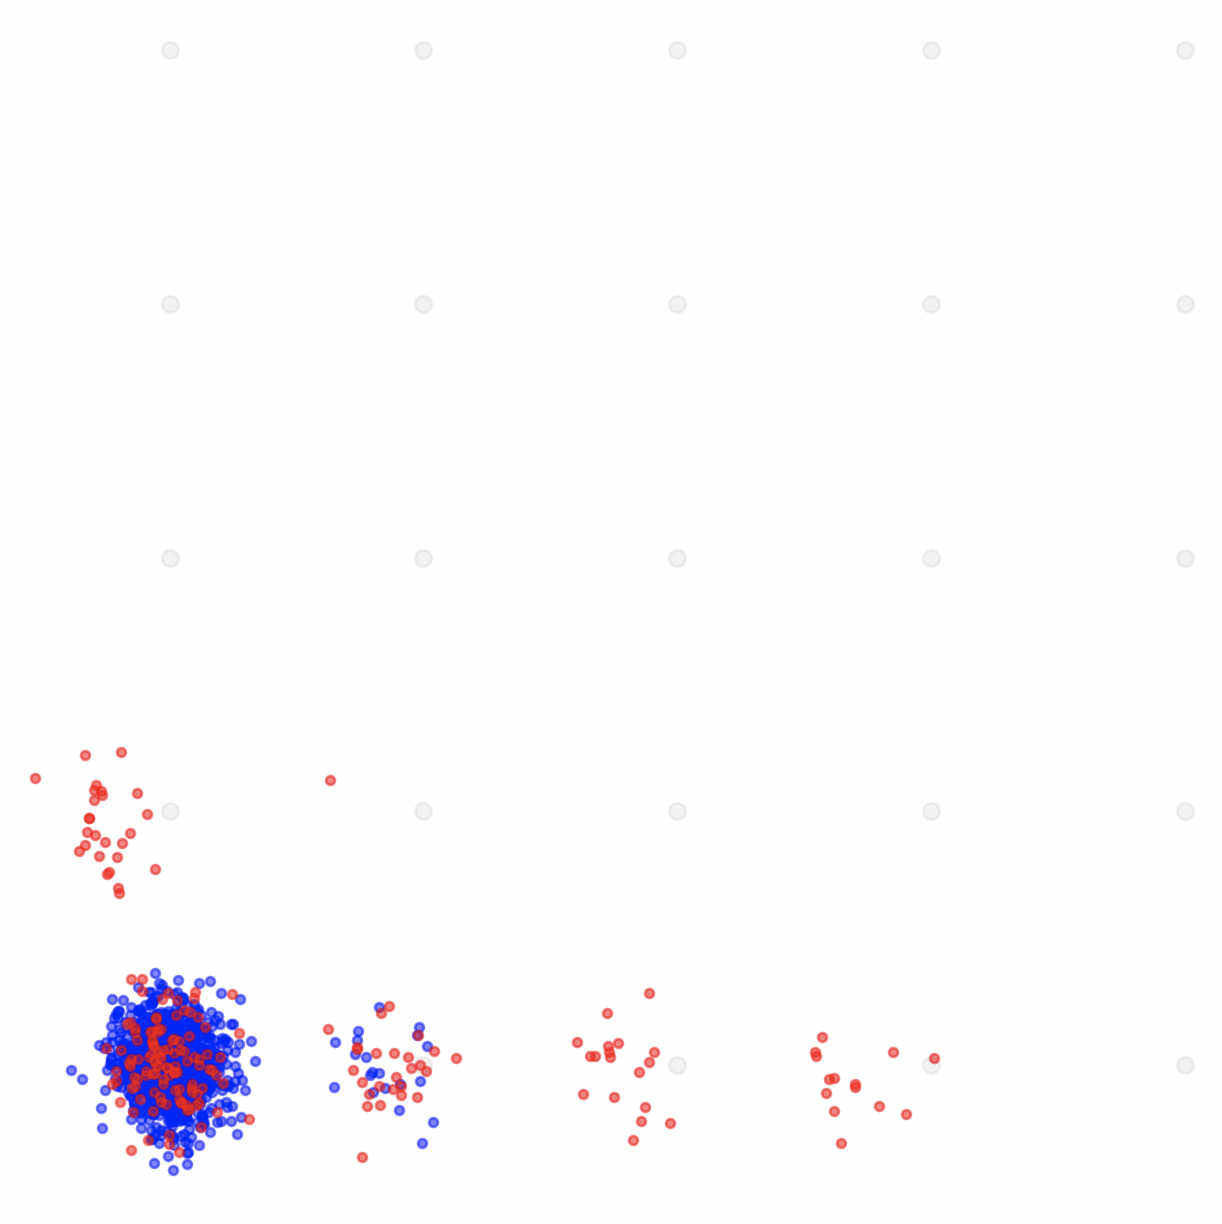
\includegraphics[width=\textwidth]{figdcps1.png}
         \caption{Observation $y_1$}
         \label{fig:y1}
     \end{subfigure}
     \hfill
     \begin{subfigure}[b]{0.45\textwidth}
         \centering
         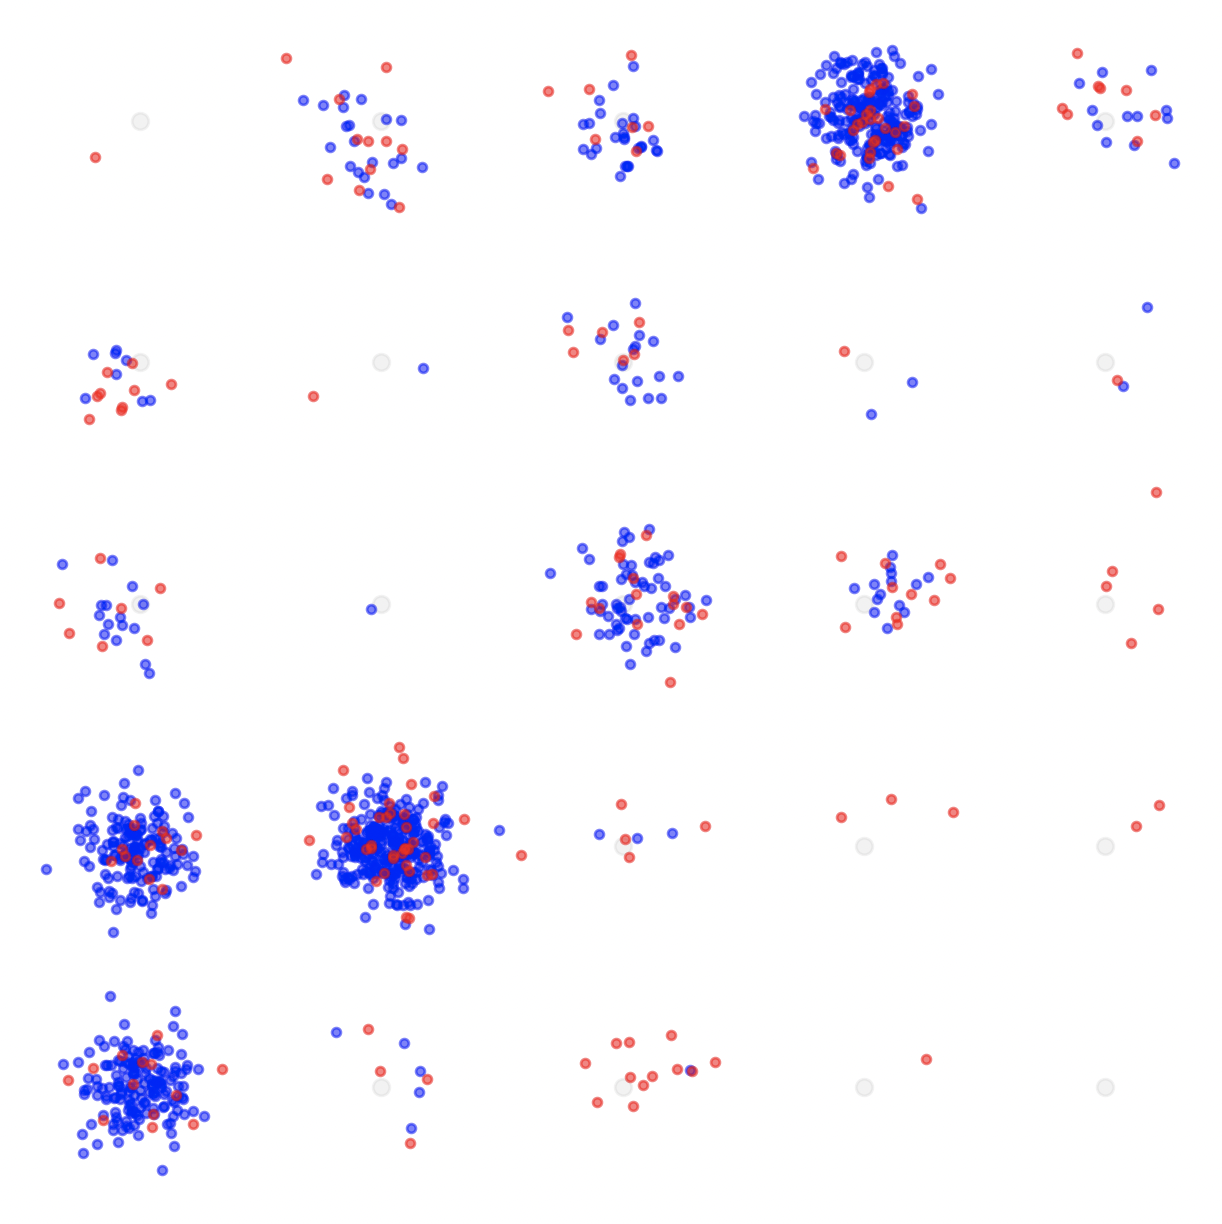
\includegraphics[width=\textwidth]{figdcps2.png}
         \caption{Observation $y_2$}
         \label{fig:y2}
     \end{subfigure}
     
     \vspace{0.5cm} % Espace vertical entre les deux lignes
     
     % Deuxième ligne
     \begin{subfigure}[b]{0.45\textwidth}
         \centering
         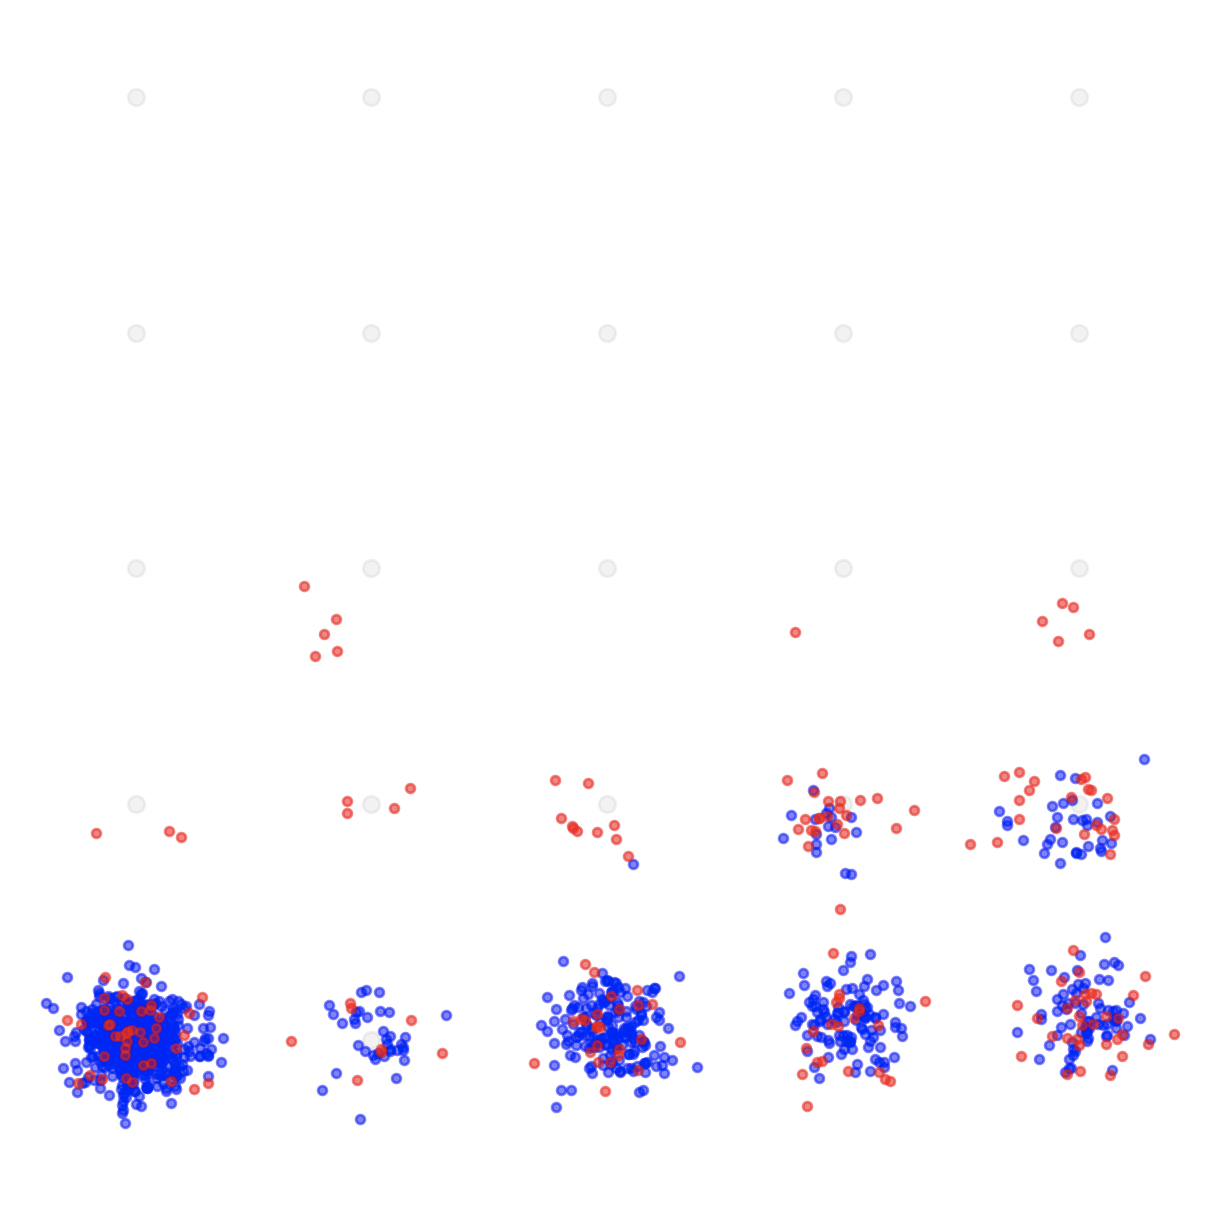
\includegraphics[width=\textwidth]{figdcps3.png}
         \caption{Observation $y_3$}
         \label{fig:y3}
     \end{subfigure}
     \hfill
     \begin{subfigure}[b]{0.45\textwidth}
         \centering
         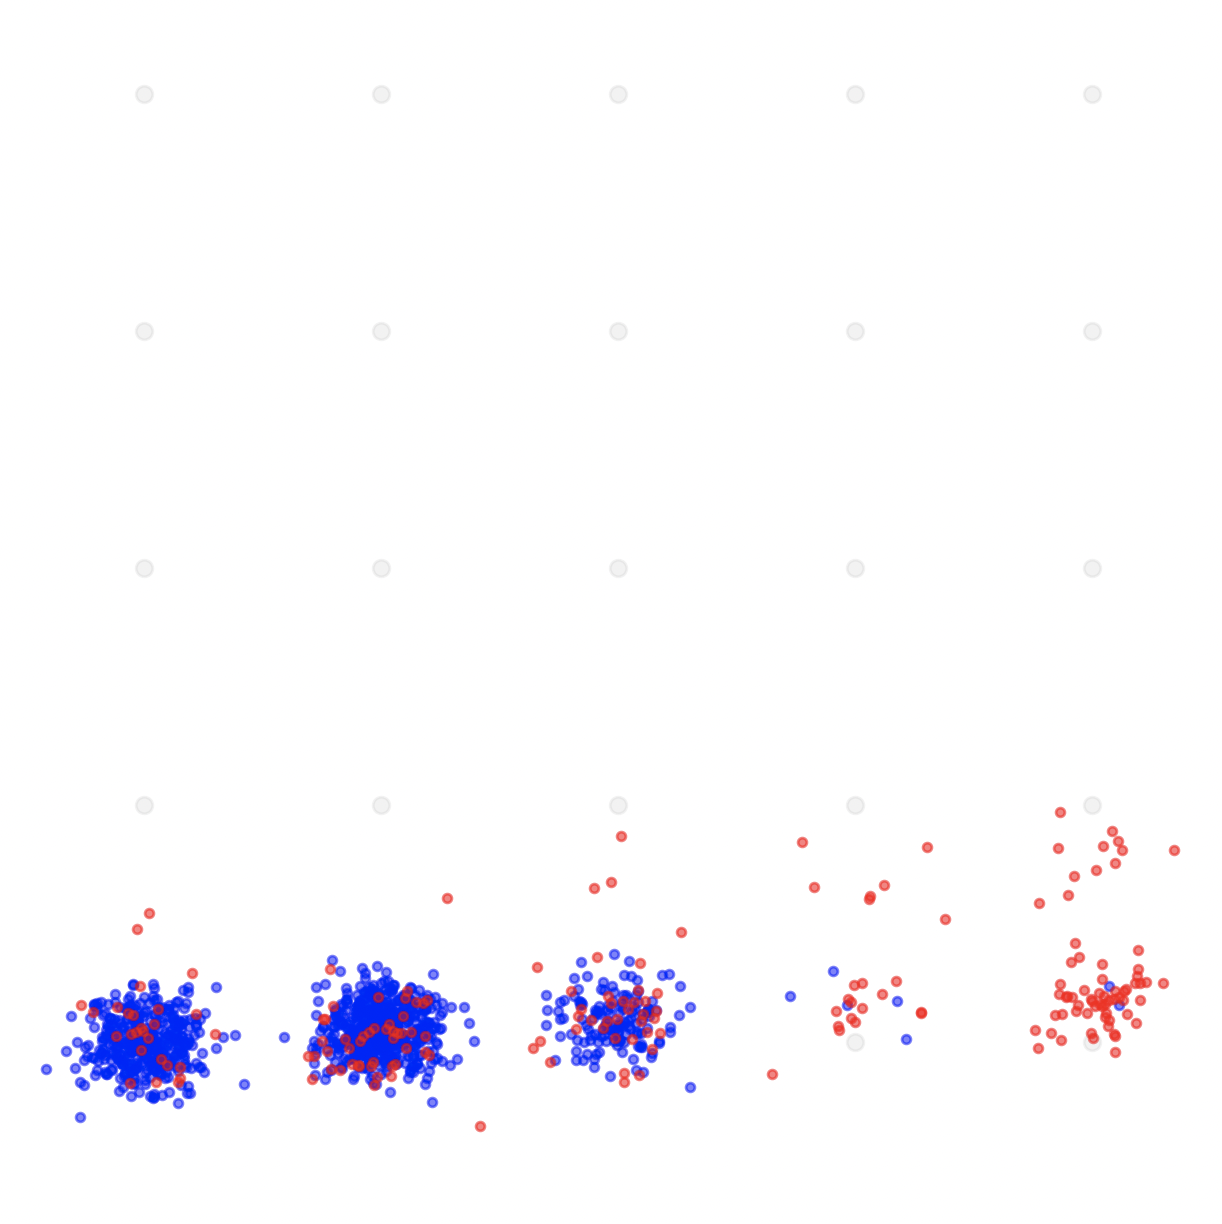
\includegraphics[width=\textwidth]{figdcps4.png}
         \caption{Observation $y_4$}
         \label{fig:y4}
     \end{subfigure}
     
     \caption{Samples generated by DCPS for four different observations in a GMM setting.}
     \label{fig:dcps_gmm_samples}
\end{figure}

\section{Usefull results on gaussians}

\begin{lemma}[Tweedie's formula]
    \label{lem:tweedie}
    Let $X$ be a random variable on $\mathbb{R}^d$ with density $p_X$. Let $Z$ be
    a random variable such that $Z | X = x \sim \mathcal{N}(x, \sigma^2 I_d)$ for some $\sigma > 0$.
    Let $p_Z$ be the density of $Z$. Then, for almost all $z \in \mathbb{R}^d$, we have
    $$\mathbb{E}[X | Z = z] = z + \sigma^2 \nabla_z \log p_Z(z).$$
\end{lemma}

\begin{proof}
    The marginal density of $Z$ is given by
    $$p_Z(z) = \int p_X(x) p_{Z|X}(z | x) dx = \int p_X(x) \frac{1}{(2 \pi \sigma^2)^{d/2}} 
    \exp\left(-\frac{\|z - x\|^2}{2 \sigma^2}\right) dx.$$
    Thus $\nabla_z p_Z(z) = \int p_X(x) \frac{-(z - x)}{\sigma^2} p_{Z|X}(z | x) dx$,
    and we have
    \begin{align*}
        \nabla_z \log p_Z(z) 
        & = \frac{\nabla_z p_Z(z)}{p_Z(z)} \\
        & = \frac{1}{p_Z(z)} \int p_X(x) \frac{-(z - x)}{\sigma^2} p_{Z|X}(z | x) dx \\
        & = \frac{1}{\sigma^2} \left( \int x \frac{p_X(x) p_{Z|X}(z | x)}{p_Z(z)} dx - z \right) \\
        & = \frac{\mathbb{E}[X | Z = z] - z}{\sigma^2}.
    \end{align*}
\end{proof}

\begin{lemma}[Product of two gaussians]
    \label{lem:prod_gaussians}
    $$\int \mathcal{N}(x; \mu_1, \Sigma_1) \mathcal{N}(x; \mu_2, \Sigma_2) dx = \mathcal{N}(\mu_1; \mu_2, \Sigma_1 + \Sigma_2)$$.
\end{lemma}
\begin{proof}
Soit l'intégrale $I = \int_{\mathbb{R}^d} \mathcal{N}(x; \mu_1, \Sigma_1) \mathcal{N}(x; \mu_2, \Sigma_2) dx$. Par définition des densités gaussiennes :
$$
I = \int_{\mathbb{R}^d} \frac{1}{(2\pi)^d \sqrt{|\Sigma_1||\Sigma_2|}} \exp \left( -\frac{1}{2} \left[ \|x-\mu_1\|_{\Sigma_1}^2 + \|x-\mu_2\|_{\Sigma_2}^2 \right] \right) dx
$$
Posons
\begin{align*}
Q(x) &= (x-\mu_1)^\top \Sigma_1^{-1} (x-\mu_1) + (x-\mu_2)^\top \Sigma_2^{-1} (x-\mu_2) \\
&= x^\top (\Sigma_1^{-1} + \Sigma_2^{-1}) x - 2x^\top (\Sigma_1^{-1}\mu_1 + \Sigma_2^{-1}\mu_2) + \mu_1^\top \Sigma_1^{-1} \mu_1 + \mu_2^\top \Sigma_2^{-1} \mu_2
\end{align*}
Posons $\Sigma_c^{-1} = \Sigma_1^{-1} + \Sigma_2^{-1}$ et $\mu_c = \Sigma_c (\Sigma_1^{-1}\mu_1 + \Sigma_2^{-1}\mu_2)$. En complétant le carré en $x$, on obtient :
$$
Q(x) = (x-\mu_c)^\top \Sigma_c^{-1} (x-\mu_c) + K
$$
Le terme constant $K$ est donné par :
\begin{align*}
K &= \mu_1^\top \Sigma_1^{-1} \mu_1 + \mu_2^\top \Sigma_2^{-1} \mu_2 - \mu_c^\top \Sigma_c^{-1} \mu_c\\
&= \mu_1^\top \Sigma_1^{-1} \mu_1 + \mu_2^\top \Sigma_2^{-1} \mu_2 
- (\Sigma_1^{-1}\mu_1 + \Sigma_2^{-1}\mu_2)^\top \Sigma_c (\Sigma_1^{-1}\mu_1 + \Sigma_2^{-1}\mu_2) \\
&= \mu_1^\top \Sigma_1^{-1} \mu_1 + \mu_2^\top \Sigma_2^{-1} \mu_2
- \mu_1^\top \Sigma_1^{-1} \Sigma_c \Sigma_1^{-1} \mu_1
- \mu_2^\top \Sigma_2^{-1} \Sigma_c \Sigma_2^{-1} \mu_2
- 2 \mu_1^\top \Sigma_1^{-1} \Sigma_c \Sigma_2^{-1} \mu_2\\
&= \mu_1^\top \left( \Sigma_1^{-1} - \Sigma_1^{-1} \Sigma_c \Sigma_1^{-1} \right) \mu_1 
+ \mu_2^\top \left( \Sigma_2^{-1} - \Sigma_2^{-1} \Sigma_c \Sigma_2^{-1} \right) \mu_2
- 2 \mu_1^\top \Sigma_1^{-1} \Sigma_c \Sigma_2^{-1} \mu_2
\end{align*}
Or 
\begin{align*}
 & \Sigma_1^{-1} - \Sigma_1^{-1}(\Sigma_1^{-1} + \Sigma_2^{-1})^{-1}\Sigma_1^{-1} = (\Sigma_1 + \Sigma_2)^{-1}\\
 & \Sigma_2^{-1} - \Sigma_2^{-1}(\Sigma_1^{-1} + \Sigma_2^{-1})^{-1}\Sigma_2^{-1} = (\Sigma_1 + \Sigma_2)^{-1}\\
& - \Sigma_1^{-1}(\Sigma_1^{-1} + \Sigma_2^{-1})^{-1}\Sigma_2^{-1} = -(\Sigma_1 + \Sigma_2)^{-1}
\end{align*}
Donc 
$$K = (\mu_1 - \mu_2)^\top (\Sigma_1 + \Sigma_2)^{-1} (\mu_1 - \mu_2)$$
L'intégrale devient alors :
\begin{align*}
I &= \frac{e^{-K/2}}{(2\pi)^d \sqrt{|\Sigma_1||\Sigma_2|}} \int_{\mathbb{R}^d} \exp \left( -\frac{1}{2} (x-\mu_c)^\top \Sigma_c^{-1} (x-\mu_c) \right) dx \\
&= \frac{e^{-K/2}}{(2\pi)^d \sqrt{|\Sigma_1||\Sigma_2|}} \cdot (2\pi)^{d/2} \sqrt{|\Sigma_c|} \\
&= \frac{1}{(2\pi)^{d/2} \sqrt{\frac{|\Sigma_1||\Sigma_2|}{|\Sigma_c|}}} \exp \left( -\frac{1}{2} (\mu_1 - \mu_2)^\top (\Sigma_1 + \Sigma_2)^{-1} (\mu_1 - \mu_2) \right)
\end{align*}

En utilisant la propriété du déterminant $|\Sigma_1||\Sigma_2||\Sigma_c^{-1}| = |\Sigma_1||\Sigma_2||\Sigma_1^{-1} + \Sigma_2^{-1}| = |\Sigma_1 + \Sigma_2|$, nous obtenons enfin :

$$I = \frac{1}{(2\pi)^{d/2} \sqrt{|\Sigma_1 + \Sigma_2|}} \exp \left( -\frac{1}{2} (\mu_1 - \mu_2)^\top (\Sigma_1 + \Sigma_2)^{-1} (\mu_1 - \mu_2) \right).$$
\end{proof}

\begin{lemma}[Distance between coupling of gaussians]
    Let $\epsilon \sim \mathcal{N}(0, I_d)$, $\mu_1, \mu_2 \in \mathbb{R}^d$ 
    and $\sigma_1, \sigma_2 \in \mathbb{R}_+^*$.
    Let $X$ and $Y$ be random variables such that
    $$X = \mu_1 + \sigma_1 \epsilon, \quad \quad Y = \mu_2 + \sigma_2 \epsilon.$$
    Then,
    $\mathbb{E} \left[ \| X - Y \|^2 \right] = \| \mu_1 - \mu_2 \|^2 + d (\sigma_1 - \sigma_2)^2$.
\end{lemma}

\begin{proof}
    We have
    \begin{align*}
        \mathbb{E} \left[ \| X - Y \|^2 \right] 
        & = \mathbb{E} \left[ \| (\mu_1 - \mu_2) + (\sigma_1 - \sigma_2) \epsilon \|^2 \right] \\
        & = \mathbb{E} \left[ \| \mu_1 - \mu_2 \|^2 + 2 (\mu_1 - \mu_2)^\top (\sigma_1 - \sigma_2) \epsilon 
        + (\sigma_1 - \sigma_2)^2 \| \epsilon \|^2 \right] \\
        & = \| \mu_1 - \mu_2 \|^2 + 0 + (\sigma_1 - \sigma_2)^2 \mathbb{E}[\| \epsilon \|^2] \\
        & = \| \mu_1 - \mu_2 \|^2 + d (\sigma_1 - \sigma_2)^2.
    \end{align*}
\end{proof}

\begin{lemma}[KL divergence between gaussians distributions]
    \label{lem:kl_gaussians}
    Let $\mu_1, \mu_2 \in \mathbb{R}^d$ and $\Sigma_1, \Sigma_2$ 
    be two positive definite matrices in $\mathbb{R}^{d \times d}$.
    Let $P_1 = \mathcal{N}(\mu_1, \Sigma_1)$ and $P_2 = \mathcal{N}(\mu_2, \Sigma_2)$
    be two Gaussian distributions.
    Then,
    \begin{equation}
    KL(P_1 || P_2) = \frac{1}{2} \left[ \text{tr}(\Sigma_2^{-1} \Sigma_1) + 
    (\mu_2 - \mu_1)^\top \Sigma_2^{-1} (\mu_2 - \mu_1) - d + \log\left(\frac{|\Sigma_2|}{|\Sigma_1|}\right) \right].
    \end{equation}
\end{lemma}

\begin{proof}
    Straightforward calculations.
\end{proof}


\end{document}